\documentclass[12pt,a4paper,twoside]{article}
\usepackage{geometry}
\geometry{a4paper}

\usepackage{amsmath}
\usepackage{amssymb}
\usepackage[utf8]{inputenc} %kompilowanie polskich literek
\usepackage[OT1]{fontenc} %wyświetlanie polskich literek
\usepackage{polski} %wyświetlanie polskich literek cz. II
\usepackage[english,polish]{babel} %zasady łamania wierszy, domyślnie polski
\usepackage{graphicx} %wstawianie obrazków
\usepackage{epstopdf} %wstawianie obrazków w formacie .eps
\usepackage{setspace}
\usepackage{fancyhdr} %nagłówki i stopki na każdej stronie
\usepackage{enumitem}
\usepackage{microtype}
\usepackage{hyperref} %możliwość linkowania
\usepackage{floatrow} %domyślnie wyśrodkowuj ryciny
\usepackage{mathtools} %\ceil, \floor
\usepackage[title]{appendix} %wsparcie dla sekcji "dodatki"
\usepackage{caption} %łamanie \caption na wiele linii
\usepackage{numprint} %separatory w dużych liczbach
\usepackage{pgfplots} %wykresy
\usepackage{fancyvrb} %centrowanie verbatim
\usepackage{xcolor} %kolory w kodzie
\usepackage{listings} %zrzuty kodów
\usepackage{textcomp} %konwersja apostrofów w zrzutach kodów
\usepackage{censor} %cenzura wulgaryzmów w badaniach
\usepackage{multicol} %środowisko dwukolumnowe
\usepackage{tikz-cd} %środowisko tikzcd (fajne strzałki)
\usepackage{datetime} %\today
\usepackage{multirow} %wiele wierszy w tabelkach

\pgfplotsset{compat=1.5} %wersja biblioteki do wykresów; usuwa problemy
\newcounter{wlcounter} %licznik list słów
\newcounter{sccounter} %licznik kodów źródłowych

%usuń kiczowate ramki dookoła linków
\definecolor{dark-red}{rgb}{0.4,0.15,0.15}
\definecolor{dark-blue}{rgb}{0.15,0.15,0.4}
\definecolor{medium-blue}{rgb}{0,0,0.5}
\hypersetup{
    colorlinks, linkcolor={dark-red},
    citecolor={dark-blue}, urlcolor={medium-blue}
}

\expandafter\def\expandafter\UrlBreaks\expandafter{\UrlBreaks\do\-}

\begin{document}
\newgeometry{margin=3cm}
\marginparwidth2.5cm
\onehalfspacing
\newcommand{\myparagraph}[1]{\paragraph{#1}\mbox{}\\}
\newcommand{\latin}[1]{\foreignlanguage{latin}{\textit{#1}}}
\newcommand{\en}[1]{\textit{\enn{#1}}}
\newcommand{\enn}[1]{\foreignlanguage{english}{#1}}
\newcommand{\abbr}[1]{\textit{#1}}
\newcommand{\renmich}[1]{\textbullet{}\marginpar{\tiny \raggedright renmich{}: #1}}
\newenvironment{myenumerate}
    {\begin{enumerate}[label*=\arabic*.]}
    {\end{enumerate}}
\DeclarePairedDelimiter{\ceil}{\lceil}{\rceil}
\DeclarePairedDelimiter{\floor}{\lfloor}{\rfloor}

\definecolor{codebg}{HTML}{EEEEEE}
\lstset{backgroundcolor=\color{codebg}}
\lstset{showstringspaces=false}
\lstset{keepspaces=true}
\lstset{tabsize=2}
\lstset{stepnumber=1}
\lstset{numbers=left}
\lstset{numbersep=5pt}
\lstset{numberstyle=\small\color{black}}
\lstset{postbreak=\raisebox{0ex}[0ex][0ex]{\ensuremath{\color{gray}\hookrightarrow\space}}}
\lstset{breaklines=true}
\lstset{keywordstyle=\color{olive}}
\lstset{stringstyle=\color{red}}
\lstset{basicstyle=\ttfamily\small}
\lstset{upquote=true}

\begin{titlepage}
    \begin{center}
    {\LARGE Uniwersytet im. Adama Mickiewicza w~Poznaniu \\
    Wydział Matematyki i~Informatyki}
    \line(1,0){350}

    \vspace{1cm}
    \includegraphics[width=3cm]{img/logo_uam.eps}
    \vspace{1cm}

    \vspace{1cm}
    {\Huge Ataki na kryptograficzne \\ funkcje skrótu} \\[0.5cm]
    {\Large Marcin Kurczewski}
    \end{center}

    \vspace{3cm}
    \hspace{8cm}\parbox[l]{6cm}{\Large Praca magisterska \\
    napisana pod kierunkiem \\
    dr Michała Rena}

    \begin{center}
    \vspace{4cm}
    Poznań, \today
    \end{center}
\end{titlepage}


\newpage
\thispagestyle{empty}
\begin{center}
    OŚWIADCZENIE
\end{center}

Ja, niżej podpisany Marcin Kurczewski, student Wydziału Matematyki
i~Informatyki Uniwersytetu im. Adama Mickiewicza oświadczam, że przedkładaną
pracę dyplomową pt.: \renmich{zły cudzysłów}``Ataki na kryptograficzne funkcje skrótu'' napisałem
samodzielnie. Oznacza to, że przy pisaniu pracy, poza niezbędnymi
konsultacjami, nie korzystałem z~pomocy innych osób, a~w~szczególności nie
zlecałem opracowania rozprawy lub jej części innym osobom, ani nie odpisywałem
tej rozprawy lub jej części od innych osób.

Oświadczam również, że egzemplarz pracy dyplomowej w~formie wydruku
komputerowego jest zgodny z~egzemplarzem pracy dyplomowej w~formie
elektronicznej.

Jednocześnie przyjmuję do wiadomości, że gdyby powyższe oświadczenie okazało
się nieprawdziwe, decyzja o~wydaniu mi dyplomu zostanie cofnięta.


\newpage
\setcounter{tocdepth}{3}
\tableofcontents

\newpage
\pagestyle{fancy}
\fancyhead[L]{\fontsize{10}{0}\selectfont
    Ataki na kryptograficzne funkcje skrótu}
\fancyhead[R]{\fontsize{10}{0}\selectfont
    Marcin Kurczewski}


\include{section1}
\section{Wprowadzenie do tematyki}



\subsection{Terminologia użyta w~pracy}
Zgodnie z~terminologią stosowaną w~kryptologii, w~pracy konsekwentnie
wykorzystywane będą następujące pojęcia:

\begin{itemize}

    \item \textbf{funkcja haszująca}~-- stosowane zamiennie z~\emph{funkcją
    skrótu},

    \item \textbf{bezpieczna funkcja haszująca}~-- stosowane zamiennie
    z~\emph{kryptograficzną funkcją skrótu},

    \item \textbf{zwykła funkcja haszująca}~-- funkcja skrótu, która może, ale
    nie musi być \emph{kryptograficzną funkcją skrótu},

    \item \textbf{wiadomość}~-- argument \emph{funkcji skrótu},

    \item \textbf{skrót}~-- wynik \emph{funkcji skrótu},

    \item \textbf{hasz}~-- stosowanie zamiennie ze \emph{skrótem},

    \item \textbf{kolizja}~-- sytuacja, w~której skróty dwóch różnych
    wiadomości są takie same, tj.
    \[
        \begin{aligned}
        m &\neq m' \\
        H(m) &= H(m')
        \end{aligned}
    \]

    \item \textbf{zadanie praktycznie niewykonalne}~-- algorytm, który
    realizuje dane zadanie nie istnieje, albo jego koszt obliczeniowy lub
    pamięciowy jest tak wielki, że nie można go wykonać przy pomocy znanych
    obecnie technologii.

\end{itemize}



\subsection{Definicja zwykłej oraz kryptograficznej funkcji skrótu}
Funkcja skrótu jest to funkcja, której dziedziną są ciągi bitów dowolnej
długości, a~przeciwdziedziną~-- ciągi bitów o~stałej, ograniczonej długości.
Rzutowanie to odbywa się w~sposób jednoznaczny, tj. każdemu wejściu funkcja
skrótu przyporządkowuje dokładnie jedno wyjście; ściślej:

$$ f \colon X \to Y $$
$$ Y \subseteq \mathbb{Z}_2^{n} : n \in \mathbb{N}$$
$$ \forall_{y \in Y} \; \exists_{x \in X} \; f(x)=y $$

\begin{figure}[htb!]
    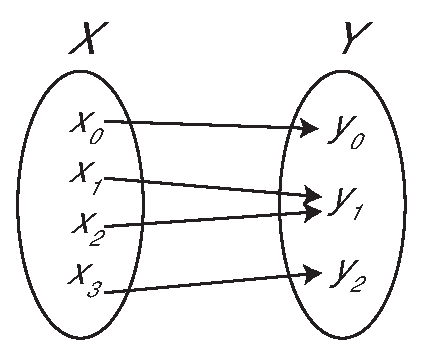
\includegraphics[width=6cm]{img/surjection.eps}
    \caption{Każdemu wejściu przyporządkowywane jest dokładnie jedno wyjście}
    \label{fig:surjection}
\end{figure}

Kryptograficzna funkcja skrótu to taka funkcja skrótu, która może być
wykorzystywana w~zastosowaniach kryptograficznych, a~więc wymagających
wysokiego poziomu bezpieczeństwa. Przykłady takich zastosowań można znaleźć
w~sekcji~\ref{sec:secure_hash_usages}. Dokładne cechy, jakie powinna spełniać
funkcja skrótu, aby była kryptograficzna, omówione zostały w~sekcji
~\ref{sec:secure_hash_attributes}. Ponadto wszystkie funkcje skrótu,
niezależnie od swojego zastosowania w~celach kryptograficznych, powinny
spełniać własności opisane w~sekcji~\ref{sec:common_hash_attributes}.



\subsubsection{Cechy zwykłych funkcji haszujących}
\label{sec:common_hash_attributes}%
Niezależnie od swojego zastosowania, każda funkcja haszująca musi spełniać
pewne warunki, które zostały poniżej opisane.

\myparagraph{Determinizm}
Funkcje haszujące powinny być deterministyczne w~takim sensie, że ich wyniki
zależą wyłącznie od danych wejściowych, a~nie żadnych czynników losowych.
Innymi słowy, haszowanie wiadomości $m$ powinno dawać taki sam skrót
niezależnie od okoliczności. Stąd wynika, że funkcje skrótu nie powinny się
nigdy odwoływać do generatorów liczb pseudolosowych, metadanych o~wiadomości
(typu jej lokalizacja w~pamięci komputera) itp., a~jedynie do samej wiadomości.

\myparagraph{Jednostajność}
Niech $H : A \to B$ będzie funkcją haszującą. Funkcje haszujące powinny
przekształcać wartości ze zbioru wejściowego $A$ na wartości ze zbioru
wyjściowego $B$ w~taki sposób, by:
\[
    \forall_{a \in A} \; \Pr(H(a) = b) \to \frac{1}{|B|}
\]
Innymi słowy dobra funkcja haszująca przekształca konkretną wartość $a$
w~konkretną wartość $b$ z~prawdopodobieństwem jak najbliższym
prawdopodobieństwu losowego wybrania tego elementu ze zbioru $B$, lub też~--
dla danej wiadomości $m$ wszystkie wartości ze zbioru $B$ powinny mieć możliwie
taką samą szansę na wybranie (z zachowaniem własności determinizmu). Cecha ta
ma na celu zapewnienie jak najmniejszego prawdopodobieństwa zajścia kolizji.

Unikanie kolizji, obok determinizmu, jest jedną z~najważniejszych cech funkcji
skrótu, co staje się zrozumiałe, gdy pozna się ich zastosowania (przykładowe
zastosowania bezpiecznych funkcji skrótu opisane są
w~sekcji~\ref{sec:secure_hash_usages}).



\subsubsection{Cechy kryptograficznych funkcji haszujących}
\label{sec:secure_hash_attributes}%
Aby lepiej zrozumieć naturę warunków nałożonych na cechy kryptograficznych
(czyli \emph{bezpiecznych}) funkcji skrótu, należy uświadomić sobie ich naturę:
w~sytuacji, kiedy kolizje są tylko niepożądane, sięgamy po zwykłe funkcje
haszujące, funkcje kryptograficzne stają się natomiast potrzebne wówczas, gdy
kolizje są \emph{niedopuszczalne}.

Jednak, z~racji mniejszego rozmiaru przeciwdziedziny w~stosunku do dziedziny
(patrz rysunek~\ref{fig:surjection} na stronie \pageref{fig:surjection}),
kolizje \emph{będą} się zdarzać.

Poniższe warunki zostały sformułowane po to, aby sytuacje, w~których dochodzi
do kolizji, były jak najmniej prawdopodobne i~żeby było trudno je celowo
wywołać, a~także żeby same kryptograficzne funkcje skrótu stanowiły godne
użycia narzędzie we wszystkich sytuacjach, które wymagają wysokiego
bezpieczeństwa.

\myparagraph{Odporność na kolizje pierwszego rzędu (\en{preimage resistance})}
\label{sec:preimage_resistance}%
Mając dany skrót $h$, znalezienie wiadomości $m$ takiej, że $H(m) = h$ powinno
być w~praktyce niewykonalne. Jest to warunek zapewniający jednostronność
bezpiecznej funkcji skrótu. Należy zauważyć, że zależy nam na \emph{dowolnej}
wiadomości, a~nie oryginalnej wiadomości z~której zostało utworzone $h$.

\myparagraph{Odporność na kolizje drugiego rzędu (\en{second preimage
resistance})}
\label{sec:second_preimage_resistance}%
Mając daną wiadomość $m$, znalezienie wiadomości $m' \neq m$ takiej, że $H(m) =
H(m')$ powinno być praktycznie niewykonalne.

\myparagraph{Odporność na kolizje (\en{collision resistance})}
\label{sec:collision_resistance}%
Znalezienie dwóch dowolnych różnych wiadomości $m \neq m'$ takich, że $H(m) =
H(m')$ powinno być praktycznie niewykonalne. Spełnienie tej własności implikuje
odporność na kolizje drugiego rzędu, ale zarazem nie gwarantuje odporności na
kolizje pierwszego rzędu.

\myparagraph{Niemożność odróżnienia od \en{random oracles}}
\en{Random oracle} to teoretyczna czarna skrzynka przypisująca każdemu
argumentowi losową (z jednostajnym rozkładem prawdopodobieństwa) wartość
z~określonej przeciwdziedziny w~taki sposób, że dla konkretnego argumentu
zawsze wybiera taką samą wartość. Pożądane jest, by kryptograficzna funkcja
skrótu była trudna do odróżnienia od \en{random oracle}~\cite{random_oracle},
choć jest to zadanie znacznie trudniejsze od zapewnienia poprzednich własności.

\myparagraph{Własność efektu lawinowego}
\label{sec:avalance_effect}%
W~kryptograficznych funkcjach haszujących powinien zachodzić tzw. efekt
lawinowy. Jest to własność zapewniająca, że nawet mała zmiana wiadomości $m'$
w~stosunku do $m$ powoduje duże zmiany w~wartości $H(m')$ w~porównaniu do
$H(m)$. Jej celem jest zapewnienie drugiej z~dwóch fundamentalnych własności
dobrego systemu kryptograficznego, sformułowanych przez Shannona
w~1949~\cite{confusion_diffusion}:

\begin{itemize}

    \item \en{confusion} (zamieszanie) -- zależność między szyfrogramem
    a~kluczem symetrycznym powinna być jak najbardziej skomplikowana
    i~nieprzewidywalna,

    \item \en{diffusion} (rozpraszanie) -- zależność między szyfrogramem
    a~tekstem jawnym powinna być jak najbardziej skomplikowana
    i~nieprzewidywalna.

\end{itemize}

Spełnienie tych warunków utrudnia potencjalne ataki.

\noindent Mówi się o~dwóch, wymienionych poniżej, kryteriach efektu
lawinowego~\cite{avalanche_criterion1,avalanche_criterion2}.

\begin{myenumerate}

    \item Ścisłe kryterium lawinowe (\en{strict avalanche criterion},
    \abbr{SAC}): po zmianie dowolnego bitu wejścia, każdy bit wyjścia powinien
    się zmienić z~prawdopodobieństwem równym $\frac{1}{2}$.

    Formalnie funkcja $f : \mathbb{Z}_2^n \to \mathbb{Z}_2^m$ spełnia ścisłe
    kryterium lawinowe, gdy:

    $$\forall i \; \sum_{x \in \mathbb{Z}_2^n} D_H(f(x) \oplus f(x \oplus
    C_i^n)) = m 2^{n-1}$$

    gdzie $D_H$ oznacza odległość Hamminga, a~$C_i^n$ oznacza $i$-ty wiersz
    macierzy identyczności $I$ (czyli wektor złożonych z~1 na $i$-tym miejscu
    i~0 na pozostałych miejscach).

    \item Kryterium niezależności bitowej (\en{bit independence criterion},
    \abbr{BIC}): po zmianie dowolnego bitu wejścia, każde dwa bity wyjścia
    powinny zmieniać się w~sposób niezależny od siebie.

    Możliwe jest ocenienie stopnia, w~jakim dana funkcja $f$ spełnia kryterium
    niezależności bitowej. Formalnie:

    $$\textrm{BIC}(f) = \max_{x, y \in \mathbb{Z}_2^n} \left( \max_{1 \leq i
    \leq n} |\textrm{corr}(f(x) \oplus (f(x) \oplus C_i^n), f(y) \oplus (f(y)
    \oplus C_i^n))| \right)$$

    gdzie $\textrm{corr}(X,Y)$ to współczynnik korelacji między zmienną $X$
    a~$Y$. W~najlepszym wypadku $\textrm{BIC}(f) = 0$, w~najgorszym
    $\textrm{BIC}(f) = 1$.

\end{myenumerate}

\begin{figure}[hbt!]
    \pgfplotsset{width=14cm,height=7cm}
    \begin{tikzpicture}
        \newcommand{\tmp}{$\Pr(H(a)_{(2,i)}=1)$}
        \begin{axis}[xlabel=$i$-ty bit skrótu
        \texttt{MD5},ylabel=\tmp,/pgf/number format/.cd,fixed,precision=3]
        \addplot[color=blue,mark=*] coordinates {
            (0, 0.501249577499)
            (1, 0.50207665441)
            (2, 0.500985834708)
            (3, 0.500601743263)
            (4, 0.498658240554)
            (5, 0.499766984524)
            (6, 0.50055309168)
            (7, 0.498996241025)
            (8, 0.50000256061)
            (9, 0.500978152879)
            (10, 0.499813075497)
            (11, 0.500092181947)
            (12, 0.500104984995)
            (13, 0.500038409144)
            (14, 0.499416181004)
            (15, 0.500189485113)
            (16, 0.500914137638)
            (17, 0.499784908791)
            (18, 0.49979515123)
            (19, 0.499108907849)
            (20, 0.499188286747)
            (21, 0.501026804462)
            (22, 0.49944690832)
            (23, 0.501011440804)
            (24, 0.500547970461)
            (25, 0.49958262063)
            (26, 0.49972345416)
            (27, 0.500340561081)
            (28, 0.500975592269)
            (29, 0.498632634458)
            (30, 0.500924380076)
            (31, 0.500058894021)
            (32, 0.499833560374)
            (33, 0.500975592269)
            (34, 0.499229256501)
            (35, 0.500862925445)
            (36, 0.499746499647)
            (37, 0.500788667766)
            (38, 0.499434105272)
            (39, 0.500023045487)
            (40, 0.500842440568)
            (41, 0.498863089324)
            (42, 0.4979259062)
            (43, 0.500245818524)
            (44, 0.499352165764)
            (45, 0.500660637285)
            (46, 0.49937521125)
            (47, 0.499946227198)
            (48, 0.499559575144)
            (49, 0.500455788514)
            (50, 0.500325197423)
            (51, 0.499492999293)
            (52, 0.499490438684)
            (53, 0.499341923325)
            (54, 0.500399455102)
            (55, 0.50075794045)
            (56, 0.499221574672)
            (57, 0.500535167413)
            (58, 0.500862925445)
            (59, 0.499869408909)
            (60, 0.501812911618)
            (61, 0.501142031895)
            (62, 0.500194606332)
            (63, 0.501666956869)
            (64, 0.501326395788)
            (65, 0.499114029068)
            (66, 0.498932225784)
            (67, 0.49992830293)
            (68, 0.499149877603)
            (69, 0.499718332941)
            (70, 0.500181803284)
            (71, 0.49868384665)
            (72, 0.498258785452)
            (73, 0.501003758975)
            (74, 0.499784908791)
            (75, 0.499211332234)
            (76, 0.499664560138)
            (77, 0.501646471992)
            (78, 0.49889381664)
            (79, 0.500637591798)
            (80, 0.499536529657)
            (81, 0.499526287218)
            (82, 0.499500681122)
            (83, 0.5010370469)
            (84, 0.500299591327)
            (85, 0.4996543177)
            (86, 0.499969272684)
            (87, 0.498530210072)
            (88, 0.499974393904)
            (89, 0.499528847828)
            (90, 0.500094742556)
            (91, 0.500094742556)
            (92, 0.499769545133)
            (93, 0.500737455573)
            (94, 0.500875728493)
            (95, 0.500722091916)
            (96, 0.500542849242)
            (97, 0.499431544662)
            (98, 0.500778425328)
            (99, 0.499244620159)
            (100, 0.499989757561)
            (101, 0.498786271035)
            (102, 0.500578697776)
            (103, 0.500169000236)
            (104, 0.499841242203)
            (105, 0.50027398523)
            (106, 0.500156197187)
            (107, 0.500640152407)
            (108, 0.499116589678)
            (109, 0.500645273627)
            (110, 0.500099863776)
            (111, 0.49951348417)
            (112, 0.499918060492)
            (113, 0.500512121926)
            (114, 0.49979515123)
            (115, 0.499669681358)
            (116, 0.500225333647)
            (117, 0.501841078324)
            (118, 0.499879651347)
            (119, 0.498970634929)
            (120, 0.500312394375)
            (121, 0.50041481876)
            (122, 0.499160120041)
            (123, 0.499188286747)
            (124, 0.49889381664)
            (125, 0.500145954749)
            (126, 0.499733696598)
            (127, 0.500734894964)
        };
        \end{axis}
    \end{tikzpicture}
    \caption{Przykładowy rozkład prawdopodobieństwa występowania ,,1'' na
    kolejnych bitach skrótów \texttt{MD5} wyrazów
    z~listy~\ref{wl:english_wordlist} w~dodatku~\ref{app:wordlists}.}
    %todo: wspomnieć o programie z dodatku C
    \end{figure}



\subsection{Zastosowania kryptograficznych funkcji skrótu}
\label{sec:secure_hash_usages}%
Same funkcje skrótu mają bardzo szerokie zastosowania, my jednak skupimy się
wyłącznie na zastosowaniach \emph{kryptograficznych} funkcji haszujących.
W~każdym przypadku opisane zastosowanie wykorzystujące podstawową cechę
kryptograficznych funkcji skrótu, jaką jest odporność na kolizje.



\subsubsection{Weryfikacja integralności danych}
\label{sec:usage_integrity_check}%
Wyobraźmy sobie sytuację, w~której użytkownik o~imieniu Alicja zmuszony jest
przetransportować jakieś dane przez niebezpieczny kanał informacji, który jest
podatny na zakłócenia, do użytkownika imieniem Bob. Niech wiadomość wysłana
przez Alicję oznaczona będzie $m$, a~wiadomość odebrana przez Boba będzie
oznaczona przez $m'$.

\begin{figure}[htb!]
    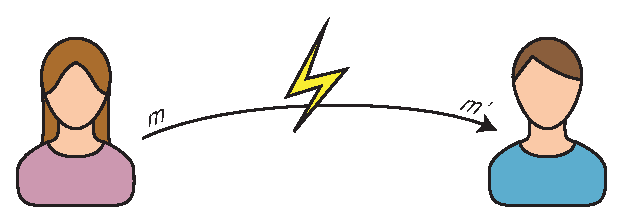
\includegraphics[width=10cm]{img/usage1.eps}
    \caption{Wiadomość odebrana przez Boba niekoniecznie musi dotrzeć do niego
    w~formie identycznej do nadanej przez Alicję}
    \label{fig:usage_integrity_check_1}
\end{figure}

Z~taką transmisją wiąże się wiele problemów, gdy zaczniemy rozpatrywać ją pod
kątem zapewnienia bezpieczeństwa. Jednym z~takim problemów jest zapewnienie
bezpiecznego mechanizmu weryfikacji, czy dane odebrane przez Boba są faktycznie
tymi samymi danymi, które były wysłane do niego przez Alicję, a~więc czy nie
zostały zmienione w~jakikolwiek sposób podczas transportu. Innymi słowy, należy
w~jakiś sposób zweryfikować, czy $m' = m$.

Z~pomocą w~rozwiązaniu tego problemu przychodzą kryptograficzne funkcje
haszujące. Alicja może, obok samej wiadomości $m$, przesłać wyliczony u~siebie
skrót tej wiadomości, $h=H(m)$. Bob może wówczas zweryfikować integralność
odebranych danych $m'$ poprzez obliczenie ich skrótu po swojej stronie
$H(m')=h'$, a~w~następnej kolejności porównanie samych skrótów (sprawdzenie,
czy obliczony przez Alicję $h$ jest równy obliczonemu przez niego $h'$).

\begin{figure}[htb!]
    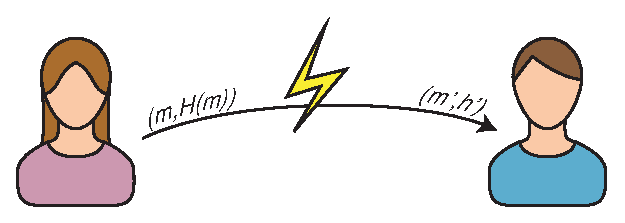
\includegraphics[width=10cm]{img/usage1b.eps}
    \caption{Bob ma teraz dodatkowy mechanizm weryfikacji integralności~--
    wystarczy, że sprawdzi, czy $H(m')=h'$.}
    \label{fig:usage_integrity_check_2}
\end{figure}

W~ten sposób wprowadzenie kryptograficznych funkcji haszujących pozwoliło
sprowadzić problem zabezpieczenia transmisji potencjalnie bardzo długich
komunikatów do zabezpieczenia transmisji jedynie samych skrótów.

Należy zdawać sobie sprawę, że nie rozwiązuje to problemu zabezpieczenia
transmisji przed rozmyślnymi atakami~-- jeśli ktoś mógł wcześniej zmieniać
zawartość $m$, teraz może również zmienić wartość $h$ zawierającą $H(m)$.
W~pewnym sensie kryptograficzne funkcje haszujące nie zapewniają żadnej
poufności danych. Mimo to z~ich zastosowania płyną pewne wymienione niżej
korzyści.

\begin{itemize}

    \item Rozwiązanie to jest przydatne w~sytuacjach, kiedy nie mamy do
    czynienia z~rozmyślnymi atakami, a~jedynie przypadkowymi zakłóceniami~--
    prawdopodobieństwo, że skrót $H(m')$ będzie równy $H(m)$ w~sytuacji, kiedy
    $m \neq m'$ będzie minimalne. Jest to jedno z~naturalnych zastosowań
    kryptograficznych funkcji haszujących, w~których odgrywają rolę trudnej do
    podrobienia sumy kontrolnej.

    \item Ponadto ułatwione jest tworzenie innych protokołów~-- dzięki funkcjom
    haszującym zależy nam na zabezpieczeniu przed modyfikacją nie całej
    wiadomości, a~jedynie jej malutkiego kawałka zawierającego skrót.
    Przykładem protokołu, który pracuje na opisanej powyżej zasadzie, jest
    podpis elektroniczny~-- \latin{de~facto} weryfikuje się tam wyłącznie
    autentyczność skrótu wiadomości, a~nie samą wiadomość.

\end{itemize}



\subsubsection{Bezpieczne przechowywanie / weryfikacja haseł}
\label{sec:usage_password_check}%
Bezpieczne funkcje haszujące przychodzą z~pomocą także w~technikach
przechowywania haseł. Wyobraźmy sobie typowy mechanizm autentykacji.

\begin{myenumerate}

    \item Użytkownik Alicja przesyła swoje dane uwierzytelniające do serwera.

    \item Serwer odbiera dane $m$.

    \item Serwer porównuje dane $m$ z~wzorcem $m'$ przechowywanym w~bazie
    danych: \label{enu:server_pass_check}

    \begin{myenumerate}

        \item jeżeli dane się zgadzają ($m = m'$), serwer udziela Alicji
        dostępu,

        \item w~przeciwnym wypadku odmawia dostępu.

    \end{myenumerate}

\end{myenumerate}

Z~takim podejściem wiążą się pewne problemy. Po pierwsze, dane, która przesyła
Alicja, mogą zostać przechwycone przez osobę trzecią, zatem wymagają
zaszyfrowania (np. poprzez zaszyfrowanie transmisji protokołem \texttt{HTTPS}).
Jednak nie ten problem okazuje się ważny z~punktu widzenia kryptograficznych
funkcji haszujących. Nas zainteresuje problem wiążący się
z~punktem~\ref{enu:server_pass_check}~-- co w~wypadku, kiedy do bazy danych
serwera, z~jakichkolwiek przyczyn, uzyskuje dostęp ktoś niepożądany? Taka osoba
może wówczas podejrzeć dane uwierzytelniające \emph{wszystkich} użytkowników,
także Alicji, a~następnie pomyślnie zalogować się przy pomocy tak wykradzionych
danych.

Musimy zatem jakoś zabezpieczyć bazę danych. Można próbować ją szyfrować lub
inaczej zabezpieczać dane w~niej przechowywane. Problemem wiążącym się z~takim
podejściem jest niestety to, że na pewnym poziomie tak czy inaczej jakaś osoba
(administrator) zawsze będzie miała dostęp do fizycznych danych. Możemy także
całkowicie zrezygnować z~przechowywania danych uwierzytelniających, a~zamiast
tego przechowywać ich skróty. Wówczas protokół podlega w~naturalny sposób
modyfikacji opisanej poniżej.

\label{sec:secure_pasword_storage}%
\begin{myenumerate}

    \item Użytkownik Alicja przesyła swoje dane uwierzytelniające do serwera.

    \item Serwer odbiera dane $m$.

    \item Serwer wylicza na ich podstawie hasz $h = H(m)$.

    \item Serwer porównuje hasz $h$ z~wzorcowym haszem $h'$ przechowywanym
    w~bazie danych:

    \begin{myenumerate}

        \item jeżeli skróty się zgadzają ($h = h'$), serwer udziela Alicji
        dostępu,

        \item w~przeciwnym wypadku odmawia dostępu.

    \end{myenumerate}

\end{myenumerate}

Dzięki temu, że w~bazie przechowywane są jedynie nieodwracalne skróty, nawet
w~przypadku kradzieży bazy danych na podstawie wykradzionych skrótów nie
powinno dać się odtworzyć oryginalnych danych (patrz
punkt~\ref{sec:preimage_resistance}). Teoretycznie zatem atakującemu taka baza
w~zasadzie do niczego się nie przyda.

Należy jednak zwrócić uwagę, że protokół ten nie jest bezpieczny bez pewnych
poprawek. Przyczyny tego problemu i~techniki wystarczające do zapewnienia
bezpieczeństwa są szczegółowo omówione w~części~\ref{sec:universal_attacks}.



\subsubsection{Jednoznaczna identyfikacja danych}
Innym zastosowaniem kryptograficznych funkcji haszujących jest identyfikacja
ciągów bajtów, a~w~szerszym ujęciu~-- plików, struktur/obiektów
programistycznych itp. Poniżej znajdują się przykłady wykorzystania tego
pomysłu w~różnego rodzaju rozwiązaniach.

\begin{itemize}

    \item Systemy kontroli wersji, w~tym Mercurial oraz Git, wykorzystują
    bezpieczne funkcje skrótu w~celu bezpiecznej identyfikacji konkretnych
    wersji pliku, numerowania kolejnych zmian i~bezpiecznego przechowywania
    historycznej struktury repozytorium.

    \item Odnośniki ed2k oraz magnet, używane w~sieciach peer-to-peer, wykorzystują
    bezpieczne funkcje skrótu w~celu lokalizacji źródeł skąd dany plik może być
    pobrany, a~także weryfikacji już ściągniętych danych (patrz
    punkt~\ref{sec:usage_integrity_check}).

    \item Struktury danych takie jak tablice mieszające (tzn. tablice, których
    kluczami może być dowolny obiekt, w~przeciwieństwie do klasycznych tablic
    o~indeksach liczbowych), wykorzystują bezpieczne funkcje haszujące do
    serializacji dowolnych obiektów do takiej postaci, jaką ich algorytmy
    indeksowania są w~stanie obsłużyć. Przykładowo, w~języku Java każdy
    zdefiniowany przez użytkownika obiekt powinien zaimplementować metodę
    \texttt{hashCode()}, która w~zamierzeniu ma pozwolić łatwo odróżniać
    (na~tyle, na~ile to możliwe) konkretne instancje obiektu w~stosunku od
    pozostałych.

\end{itemize}

\begin{figure}[bht]
    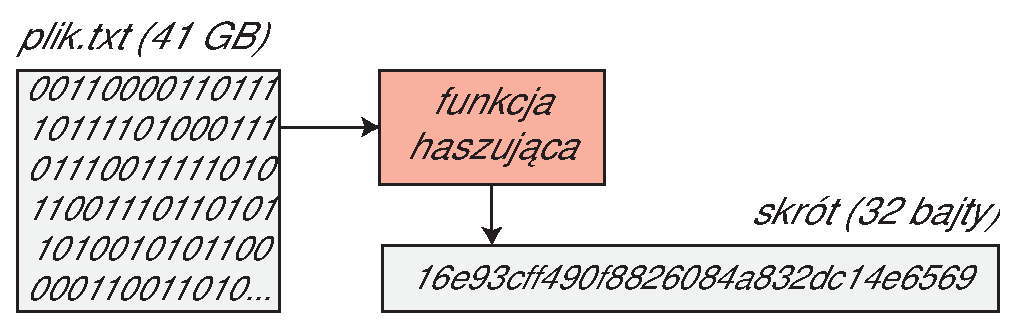
\includegraphics[width=12cm]{img/usage3.eps}
    \caption{Gdy trzeba zweryfikować poprawność przesłania dużej struktury,
    łatwiej porównać krótki skrót}
\end{figure}

Biorąc pod uwagę fakt, że kryptograficzne funkcje skrótu są dużo bardziej
kosztowne obliczeniowo niż zwykłe, nieodporne na ataki funkcje haszujące,
w~większości tego typu zastosowań korzystanie z~kryptograficznych funkcji
skrótu postrzegane jest jako przesada i~stosowane są zwyczajne funkcje skrótu.
Mimo to, czasem jednak bezpieczeństwo jest konieczne, szczególnie w~sytuacjach
opisanych powyżej, gdzie ryzyko ataku jest wysokie. Przykładowo, atakujący może
stworzyć plik zawierający wirus, którego hasz byłby taki sam jak skrót całkiem
niewinnego pliku, po czym umieścić taki plik w~sieci peer-to-peer~-- dzięki
zastosowaniu kryptograficznych funkcji skrótu, taki scenariusz jest bez
porównania trudniejszy do skutecznego przeprowadzenia.



\subsection{Rys historyczny}
Historia kryptograficznych funkcji haszujących sięga późnych lat 70--tych.
W~roku 1976 Diffie i~Hellman w~swojej pracy traktującej o~kryptografii
z~kluczem publicznym, opisali zapotrzebowanie na funkcję mapującą ciągi bitów
dowolnej długości na ciągi bitów ograniczonej długości w~nieodwracalny sposób.
W~roku 1978 Rabin po raz pierwszy zaproponował funkcję skrótu opartą na
64--bitowym wariancie blokowego algorytmu szyfrującego DES. W~1979 roku Yuval
opisał sposób, jak wykorzystując paradoks urodzinowy złamać $n$--bitową funkcję
haszującą w~czasie $2^{n/2}$.

W~tym samym roku zaczęły się pojawiać pierwsze próby zdefiniowania warunków,
jakie powinny spełniać bezpieczne funkcje skrótu. W~1979 Merkle wprowadził
pojęcie odporności na kolizje oraz odporności pierwszego i~drugiego rzędu
(patrz sekcja~\ref{sec:secure_hash_attributes}). Definicje te zostały
ostatecznie sformalizowane przez Damg\r{a}rda w~roku 1987. W~roku 2004 Rogaway
i~Shrimpton pokazali, że kryptograficzne funkcje haszujące w~miarę możliwości
nie powinny być odróżnialne od \en{random oracles}.

Już od samego początku, czyli późnych lat 70--tych\renmich{Ktoś lepszy ode mnie w typografii powinien się wypowiedzieć czy nie powinno być 70-tych. Zapytam dr Borkowskiego.}, kryptograficzne funkcje haszujące
przeżywały bardzo szybki rozwój. Zapotrzebowanie na bezpieczne i~szybkie
funkcje skrótu było szeroko rozumiane, nie zaskakuje zatem fakt, że do lat
90--tych znane było już około 50 konstrukcji. Pierwsi kandydaci korzystali
z~dorobku blokowych funkcji szyfrujących; w~późniejszym okresie rozwoju
niektórzy poszli w~kierunku teoretycznych konstrukcji opartych na algebrze
liniowej. Z~czasem jednak zaniechano adaptowania mechanizmów sprawdzonych
w~innych zastosowaniach na rzecz tworzenia dedykowanych funkcji.

Tak naprawdę do dnia dzisiejszego niewiele się zmieniło: od lat mamy do
czynienia z~ciągłym procesem wykazywania słabości istniejących rozwiązań
i~w~odpowiedzi wymyślania kolejnych usprawnień bądź całkiem nowych konstrukcji.
Proces ten zyskał nawet niedawno własne wydarzenie medialne w~postaci konkursu
ogłoszonego przez \enn{National Institute of Standards and Technology}, mającego
na celu wyłonienie następcy funkcji haszujących \texttt{SHA-1} i~\texttt{SHA-2}
spośród kilkudziesięciu kandydatów zgłoszonych przez kryptologów z~całego
świata. Cykl ten będzie prawdopodobnie trwał tak długo, aż zostanie odkryta
uniwersalna kryptograficzna funkcja skrótu lub wykazana zostanie niemożność
stworzenia takowej.

\section{Ataki uniwersalne}
\label{sec:universal_attacks}
Wprawdzie kryptograficzne funkcje haszujące z~założenia są bezpieczne, nie
oznacza to, że są one nie do złamania. Istnieje kilka ogólnych technik, które
można stosować do znajdywania oryginalnych wiadomości $m$ niezależnie od
rodzaju użytej funkcji.

\subsection{Ataki naiwne}
Wyobraźmy sobie scenariusz, w~którym z~serwera uwierzytelniającego została
wykradziona baza danych zawierająca nazwy użytkowników i~ich hasła zakodowane
dowolną funkcją haszującą. W~naiwnym podejściu atakujący może próbować zgadnąć
kolejne hasła, jakich mogli użyć użytkownicy i~porównywać hasze tych
wymyślonych haseł z~haszami z~wykradzionej bazy danych.



%todo ataki online ataki offline



\subsubsection{Atak brutalny}
W~tym podejściu konsekwentnie wypróbowywane są wszystkie hasła, jakie się da
utworzyć za pomocą danego alfabetu $A$, zwiększając długość wypróbowywanych
haseł \latin{ad infinitum}. Przykładowo, mając alfabet $A=(\mathtt{a},
\mathtt{b}, \mathtt{c}, \ldots, \mathtt{z})$ atakujący będzie próbował znaleźć
kolizje haszy dla kolejnych haseł: $\mathtt{a}, \mathtt{b}, \mathtt{c}, \ldots,
\mathtt{z}, \mathtt{aa}, \mathtt{ab}, \ldots$ itd.

Technika ta, zwana także czasem przeszukiwaniem pełnym, przy odpowiednim
alfabecie sprawia, że pomyślne znalezienie kolizji jest jedynie kwestią czasu.
Jest ona jednak wyjątkowo nieoptymalna z~uwagi na ilość zasobów, które są
potrzebne do pomyślnego przeprowadzenia. Chcąc sprawdzić wszystkie hasła
długości \mbox{$|m| \in (1, \ldots n)$} nad alfabetem długości $a=|A|$, musimy
przeprowadzić następującą liczbę operacji haszowania:
    $$\sum_{i=1}^n a^i = \frac{a(a^n-1)}{a-1}$$
Przykładowo, chcąc sprawdzić wszystkie hasła nad alfabetem składającym się
z~cyfr oraz z~małych i~wielkich znaków alfabetu łacińskiego (a~więc $|A| =
10+26+26 = 62$) o~długości od~1~do~8~znaków, musimy wypróbować następującą
liczbę możliwości:
    $$\frac{62(62^8-1)}{62-1} = \numprint{221919451578090}$$
Zakładając, że atakujący~potrafi obliczyć 100000~haszy na~sekundę, nadal
potrzebuje ok.~70~lat na złamanie hasła; jest to zatem wyjątkowo niepraktyczne
podejście i~z~reguły skazane jest na niepowodzenie.



\subsubsection{Zrandomizowany atak brutalny}
Mimo że ataki brutalne w~domyślnej formie są niepraktyczne, atakujący mogą
wprowadzić różnego rodzaju ulepszenia, tak by nie marnować czasu na
przeszukiwanie nieprawdopodobnych haseł. Jednym z~takich podejść jest
wykorzystanie zdobyczy analizy częstości: wiadomo, że w~pewnych językach pewne
litery są częściej wykorzystywane niż inne, a~większość osób nie stara się
czynić swoich haseł bezpiecznymi i~korzysta z~haseł będącymi zwykłymi słowami
istniejącymi w~jakimś języku (więcej w~sekcji~\ref{sec:dictionary_attacks}).

%todo: rozszerzyć tabelę o język polski
\begin{table}[htb]
    \caption{Przybliżony rozkład częstości występowania liter alfabetu
    łacińskiego w~języku angielskim (tabelka sporządzona na podstawie
    listy~\ref{wl:wiki_wordlist} przy użyciu skryptu~\ref{sc:ngrams_counter}).}
    \begin{tabular}{|r||c|l|}
        \hline
        &Znak & \small \small \% wystąpień \\
        \hline
        1  & e & 12.47125\% \\
        2  & t &  8.76323\% \\
        3  & a &  8.48548\% \\
        4  & i &  7.72037\% \\
        5  & o &  7.54299\% \\
        6  & n &  7.46700\% \\
        7  & s &  6.74592\% \\
        8  & r &  6.63512\% \\
        9  & h &  4.68796\% \\
        10 & l &  4.30882\% \\
        11 & d &  3.74735\% \\
        12 & c &  3.42035\% \\
        13 & u &  2.70168\% \\
        14 & m & 2.59310\% \\
        15 & f & 2.21636\% \\
        16 & p & 2.04369\% \\
        17 & g & 1.85573\% \\
        18 & y & 1.62379\% \\
        19 & w & 1.44348\% \\
        20 & b & 1.41570\% \\
        21 & v & 1.04336\% \\
        22 & k & 0.50712\% \\
        23 & x & 0.24109\% \\
        24 & z & 0.11776\% \\
        25 & q & 0.10610\% \\
        26 & j & 0.09521\% \\
        \hline
    \end{tabular}
\end{table}

Można to wykorzystać układając alfabet w~kolejności zgodnej z~kolejnością
występowania liter w~danym języku, tak by polepszyć prawdopodobieństwo
wczesnego dobrego doboru literek. Przykładowo, domyślnie korzystalibyśmy
z~alfabetu ułożonego w~następujący sposób:
    $$A_1 = (
    \mathtt{a}, \mathtt{b}, \mathtt{c}, \mathtt{d}, \mathtt{e}, \mathtt{f},
    \mathtt{g}, \mathtt{h}, \mathtt{i}, \mathtt{j}, \mathtt{k}, \mathtt{l},
    \mathtt{m}, \mathtt{n}, \mathtt{o}, \mathtt{p}, \mathtt{q}, \mathtt{r},
    \mathtt{s}, \mathtt{t}, \mathtt{u}, \mathtt{v}, \mathtt{w}, \mathtt{x},
    \mathtt{y}, \mathtt{z})$$
Dla języka angielskiego moglibyśmy natomiast ułożyć alfabet w~poniższej
kolejności:
    $$A_2 = (
    \mathtt{e}, \mathtt{t}, \mathtt{a}, \mathtt{o}, \mathtt{i}, \mathtt{n},
    \mathtt{s}, \mathtt{h}, \mathtt{r}, \mathtt{d}, \mathtt{l}, \mathtt{c},
    \mathtt{u}, \mathtt{m}, \mathtt{w}, \mathtt{f}, \mathtt{g}, \mathtt{y},
    \mathtt{p}, \mathtt{b}, \mathtt{v}, \mathtt{k}, \mathtt{j}, \mathtt{x},
    \mathtt{q}, \mathtt{z})$$
Przypuśćmy, że hasło brzmi ``thesis'' i~szukamy go metodą brutalną.
Dla zadanego alfabetu $A$, zanim znajdziemy słowo ``thesis'' trzeba wygenerować
następującą liczbę haseł:
    \[
        \begin{aligned}
        (A[\mathtt{t}]-1)\cdot(|A|^5) &+\\
        (A[\mathtt{h}]-1)\cdot(|A|^4) &+\\
        (A[\mathtt{e}]-1)\cdot(|A|^3) &+\\
        (A[\mathtt{s}]-1)\cdot(|A|^2) &+\\
        (A[\mathtt{i}]-1)\cdot(|A|^1) &+\\
        (A[\mathtt{s}]-1)\cdot(|A|^0)
        \end{aligned}
    \]
gdzie $A[x]$ oznacza pozycję litery $x$ w~alfabecie $A$ (indeksując od 1).
Korzystając z~powyższego wzoru można obliczyć ile operacji zajmie znalezienie
hasła metodą brutalną z~domyślnym alfabetem $A_1$:
    \[
        \begin{aligned}
        n_1=\;&19 \cdot 62^5 + 7 \cdot 62^4 \\
        +\;&4 \cdot 62^3 + 18 \cdot 62^2 \\
        +\;&8 \cdot 62^1 + 18 \cdot 62^0 \\
        =\;&\numprint{17510981178}
        \end{aligned}
    \]
\ldots a~ile zajmie znalezienie hasła przy pomocy mądrze spreparowanego
$A_2$:
    \[
        \begin{aligned}
        n_2=\;&1 \cdot 62^5 + 7 \cdot 62^4 \\
        +\;&0 \cdot 62^3 + 6 \cdot 62^2 \\
        +\;&4 \cdot 62^1 + 6 \cdot 62^0 \\
        =\;&\numprint{1019590502}
        \end{aligned}
    \]
Jest to ponad 17 razy krócej. Należy jednak zauważyć, że tak dobry przyrost
wynika głównie ze szczęśliwego wyboru pierwszej litery: w~pierwszym podejściu
przy najwyższej potędze występował mnożnik 19, w~drugim -- tylko 1. Widać stąd,
że przy takiej strategii im mniej używana będzie pierwsza litera faktycznego
hasła które atakujący próbuje znaleźć, tym dłuższy będzie czas jego łamania.

Powyższa obserwacja prowadzi do szukania innego sposobu na optymalizację. Tak
naprawdę zawsze, gdy przestrzeń haseł przeszukuje się liniowo, szybkość
znalezienia kolizji będzie najbardziej uzależniona od wczesnych wyborów cechy,
która jest modyfikowana (w przypadku klasycznych ataków brutalnych cechą tą
jest dobór kolejnych liter). Jest to niepożądane zjawisko, dlatego wykształciła
się inna rodzina ataków brutalnych, jaką są ataki zrandomizowane. W~tym
podejściu zamiast liniowo przeszukiwać przestrzeń haseł próbuje się je
przeszukiwać tak, by każda kombinacja miała względnie równą szansę być
wypróbowana wraz z~upływem czasu, bez znacznego faworyzowania jakichkolwiek
cech (w~szczególności bez np. faworyzowania haseł zaczynających się na
literkę~``a'', w~następnej kolejności~``aa'' itd.). Do implementacji takiego
wyszukiwania można podejść na kilka sposobów.
\begin{myenumerate}
    \item Na pierwszy rzut oka nasuwa się myśl, że można by po prostu
    wygenerowane hasła potasować. Podejście to jest jednak nieskuteczne,
    ponieważ potasowanie odbywa się tutaj dopiero \emph{po} wygenerowaniu. Nic
    tak naprawdę nie zyskujemy, a~wręcz tracimy: najpierw należy całość
    wygenerować i~przechować w~jakiejś strukturze danych, co niesie ze sobą
    ogromne koszty pamięciowe, a~następnie wykonać długotrwałą operację
    tasowania. Kluczowym elementem jest uzyskanie losowości już \emph{podczas}
    generowania tak, by nie trzeba było przechowywać wypróbowywanych haseł
    w~pamięci.

    \item W~sytuacji, kiedy chcemy osiągnąć losowy porządek już na etapie
    tworzenia listy, możemy zmienić sposób obliczania nowego hasła na podstawie
    poprzedniego. Niech $N(x, A)=y$, gdzie $x$ to poprzednie hasło, $y$ to
    nowo wygenerowane hasło a~$A$ to alfabet. W~klasycznym ataku brutalnym
    funkcja następnika dla $A=(\mathtt{a}, \mathtt{b}, \mathtt{c}, \ldots,
    \mathtt{z})$ zachowuje się następująco:
    \[
        \begin{aligned}
            N(\varnothing, A) &= \mathtt{a} \\
            N(\mathtt{a},  A) &= \mathtt{b} \\
            N(\mathtt{b},  A) &= \mathtt{c} \\
            &\vdots \\
            N(\mathtt{z},  A) &= \mathtt{aa} \\
            N(\mathtt{aa}, A) &= \mathtt{ab} \\
            &\vdots
        \end{aligned}
    \]
    W~teorii można jednak skonstruować funkcję następnika, która przyjmując
    dodatkowe parametry oznaczające minimalną i~maksymalną długość hasła,
    będzie zwracała hasła w~kolejności przypominającej losową:
    \[
        \begin{aligned}
            N(\varnothing, A, 1, 2) &= \mathtt{gx} \\
            N(\mathtt{gx}, A, 1, 2) &= \mathtt{zt} \\
            N(\mathtt{zt}, A, 1, 2) &= \mathtt{a} \\
            N(\mathtt{a}, A, 1, 2) &= \mathtt{kk} \\
            &\vdots
        \end{aligned}
    \]

    Mając taką funkcję można dowiedzieć się, jakie hasło powinno zostać
    wypróbowane w~następnej kolejności, przy zachowaniu pseudolosowego porządku
    oraz bez żadnych kosztów pamięciowych.

    Podejście to znajduje swoje korzenie w~trybach szyfrów blokowych, gdzie
    zazwyczaj zależy nam by poprzedni blok wpływał w~jak najbardziej
    nieprzewidywalny sposób na wygląd aktualnego bloku (co realizuje dowolny
    tryb inny niż \texttt{ECB}). Wadą tego rozwiązania jest to, że
    implementacja iteratora, który będzie zwracał wyniki w~kolejności
    przypominającej losową, jest trudna w~implementacji oraz kosztowna
    obliczeniowo, a~przy generowaniu haseł zależy nam na jak najoptymalniejszym
    szybkościowo i~pamięciowo działaniu procesu.

    \item Można też zwyczajnie generować przypadkowe hasła. Jest to podejście
    atrakcyjne, bo nie dość, że jest proste w~implementacji oraz tanie
    obliczeniowo (zakładając szybkość działania wykorzystanych generatorów
    liczb pseudolosowych), to zostawia także dużo miejsca na kolejne
    ulepszenia.

    Głównym problemem wiążącym się z~losowaniem haseł jest możliwość
    otrzymywania tego samego hasła wielokrotnie, dopóki nie zostanie
    wprowadzone zabezpieczenie w~postaci struktury danych zapamiętującej
    wypróbowane hasła. To jednak z~kolei oznacza wysokie koszty: pamięciowe,
    w~celu trzymania zapamiętanych haseł, oraz obliczeniowe, w~celu
    sprawdzania, czy wylosowane hasło zostało już wybrane. Zależnie od
    szybkości działania łamanej funkcji haszującej oraz charakteru ataku
    (łamanie pojedynczego hasła vs. łamanie zbioru haseł), implementowanie tego
    typu sprawdzania może być opłacalne lub nie.

    Samo generowanie losowych haseł można zrealizować kierując się różnymi
    wytycznymi. W~podejściu całkowicie losowym można po prostu składać ze sobą
    $n$ przypadkowych znaków z~alfabetu $A$. Popełnialibyśmy jednak w~ten
    sposób ten sam błąd, co wcześniej -- także i~w~tym wypadku można skorzystać
    z~dobrodziejstwa analizy~częstości i~uzależnić prawdopodobieństwa
    wyciągnięcia odpowiednich liter od prawdopodobieństwa ich wystąpienia
    w~zakładanym języku. Możemy pójść także krok dalej i~uzależnić swój
    generator od prawdopodobieństw występowania tzw. digramów oraz trigramów,
    czyli ciągów odpowiednio 2- i~3-literowych.

    \begin{table}[htb]
        \caption{Przybliżenie 15 najczęściej występujących digramów oraz
        trigramów złożonych z~liter alfabetu łacińskiego w~języku~angielskim
        (tabelka sporządzona na podstawie listy~\ref{wl:wiki_wordlist} przy
        użyciu skryptu~\ref{sc:ngrams_counter}).}
        \begin{tabular}{|r||c|l||c|l|}
            \hline
            & Bigram & \small \% wystąpień &
            Trigram & \small \% wystąpień \\
            \hline
            1  & th & 3.08514\% & the & 2.88025\% \\
            2  & he & 2.86055\% & and & 1.21997\% \\
            3  & in & 2.40712\% & ion & 0.95958\% \\
            4  & er & 2.15763\% & ing & 0.95724\% \\
            5  & an & 2.11390\% & tio & 0.76296\% \\
            6  & on & 1.77424\% & ent & 0.71174\% \\
            7  & re & 1.76263\% & ati & 0.56554\% \\
            8  & at & 1.41375\% & ter & 0.54204\% \\
            9  & ti & 1.39238\% & for & 0.48440\% \\
            10 & en & 1.38312\% & ate & 0.46068\% \\
            11 & es & 1.38072\% & her & 0.41935\% \\
            12 & or & 1.36063\% & all & 0.38966\% \\
            13 & te & 1.31308\% & ver & 0.37819\% \\
            14 & nd & 1.30632\% & ers & 0.37419\% \\
            15 & ed & 1.28358\% & ere & 0.37155\% \\
            \hline
        \end{tabular}
    \end{table}

    Wprowadzając zróżnicowane prawdopodobieństwa wyboru liter, wybór hasła
    zostaje związany z~cechą jaką jest rozkład prawdopodobieństwa liter. Jednak
    w~odróżnieniu od poprzedniej metody, faworyzowanie tym sposobem odbywa się
    w~sposób nieliniowy, co eliminuje opisaną wcześniej niechcianą stronniczość
    związaną z~wyborem pierwszych liter. Z~tego też powodu autor uważa opisaną
    w~tym punkcie metodę za lepszą od obu wcześniejszych podejść (klasyczne,
    w~którym hasło zaczynające się na ``z'' \emph{musi} czekać aż wszystkie
    inne zostaną obliczone, oraz całkowicie losowe, w~którym hasła, które
    uznane są za bardziej prawdopodobne na podstawie analizy językowej, są
    wybierane równie często jak pozostałe).

\end{myenumerate}

Analiza częstości, w~szczególności di- oraz trigramów, jest uznaną metodą
ulepszania ataku brutalnego i~wykorzystywana jest w~programach takich jak
\texttt{John The Ripper}~\cite{john_the_ripper_modes}.
\pagebreak



\subsubsection{Atak słownikowy}
\label{sec:dictionary_attacks}
Innym rodzajem ataku jest atak słownikowy. Podobnie jak omówione powyżej metody
opiera się on na wypróbowaniu kolejnych haseł, jednak w~tym przypadku zamiast
sprawdzać \emph{wszystkie} możliwe hasła, co może zająć bardzo dużo czasu,
atakujący zawęża wybór swoich kandydatów do z~góry znanego stałego zbioru
o~skończonej wielkości (czyli tytułowego słownika). Słownik powinien się
składać z~wyrazów, których użycie jako hasło przez użytkowników jest
najbardziej prawdopodobne. Mogą to być słowa w~określonym języku, imiona itp.;
tak naprawdę nawet gdy dany słownik zawiera kilkanaście milionów słów,
sprawdzanie nimi metodą ``offline'' odbywa się bardzo szybko. Atakujący mogą
także pójść krok dalej i~skorzystać z~publicznie dostępnych raportów
o~najczęściej używanych hasłach -- przykładem takiego raportu może być
lista~\ref{wl:xato_passwords}.

    \begin{table}[htb]
        \caption{Przybliżenie 15 najpopularniej stosowanych haseł przez
        użytkowników Internetu (tabelka sporządzona na podstawie
        listy~\ref{wl:xato_passwords} przy użyciu
        skryptu~\ref{sc:freq_percentages}).}
        \begin{tabular}{|r||c|c|}
            \hline
            & Hasło & \small \% wystąpień \\
            \hline
            1  & password & 1.70768\% \\
            2  & 123456   & 1.38467\% \\
            3  & 12345678 & 0.46212\% \\
            4  & 1234     & 0.30851\% \\
            5  & qwerty   & 0.29086\% \\
            6  & 12345    & 0.24117\% \\
            7  & dragon   & 0.23040\% \\
            8  & p\censor{uss}y & 0.21035\% \\
            9  & baseball & 0.19936\% \\
            10 & football & 0.19632\% \\
            11 & letmein  & 0.18854\% \\
            12 & monkey   & 0.18593\% \\
            13 & 696969   & 0.17836\% \\
            14 & abc123   & 0.17649\% \\
            15 & mustang  & 0.17537\% \\
            \hline
        \end{tabular}
    \end{table}

Dodatkowo w~przypadku gdy atakujący obiera na cel konkretny system, może on
rozszerzać swój słownik o~dodatkowe informacje kontekstowe związane
z~tym systemem. Przykładowo, dla portalu internetowego słownik może zostać
rozszerzony o~słowa kluczowe występujące na jego stronach, a~w~przypadku
zdalnych terminali o~nazwy użytkowników i~katalogów domowych.



\subsubsection{``Mutowanie'' kandydatów}
Często się zdarza tak, że na użytkownikach jest wymuszane stosowanie hasła
przykładowo zawierającego co~najmniej jedną cyfrę. W~wypadku, gdy słownik
atakującego zawiera wyłącznie kandydatów pozbawionych cyfr, słownik taki
staje się bezużyteczny. Dlatego też czasem stosuje się swoiste ``mutowanie''
kandydatów, na które przypada szereg technik przetwarzających bazowe hasło na
takie, które mogło zostać wykorzystane przez ewentualnego użytkownika.
Przykładowe techniki zostały wymienione poniżej.

\begin{itemize}

    \item
        Zmiana wielkości liter \\
        Liczba generowanych haseł: $2^n$, gdzie $n$ to długość hasła.

        \lstinputlisting[language=python,caption=Przykładowy kod
        w~Pythonie]{code/mutate_alpha.py}
        \lstinputlisting[caption=Przykładowe użycie dla
        \texttt{mutate\_alpha('abc')}]{code/mutate_alpha.txt}

    \pagebreak
    \item
        Dopisywanie cyfr na końcu hasła \\
        Liczba generowanych haseł: 11.

        \lstinputlisting[language=python,caption=Przykładowy kod
        w~Pythonie]{code/mutate_digit_end.py}
        \lstinputlisting[caption=Przykładowe użycie dla
        \texttt{mutate\_digit\_end('abc')}]{code/mutate_digit_end.txt}

    \item
        Dopisywanie znaków z~określonego zbioru w~dowolnym miejscu hasła \\
        Liczba generowanych haseł: $1 + |A| \cdot n$, gdzie $n$ to długość hasła,
        $A$ to zbiór znaków do dopisania.

        \lstinputlisting[language=python,caption=Przykładowy kod
        w~Pythonie]{code/mutate_char_insert.py}
        \pagebreak
        \lstinputlisting[caption=Przykładowe użycie dla
        \texttt{mutate\_char\_insert('abc','de',2)}]{code/mutate_char_insert.txt}

    \item
        Zamiana liter zgodnie z~tablicą możliwych podstawień \\
        Przeciętna liczba generowanych haseł jest zależna od rozkładu częstości
        liter w~słowniku używanych przez tablicę podstawień.

        \lstinputlisting[language=python,caption=Przykładowy kod
        w~Pythonie]{code/mutate_char_sub.py}

        \lstinputlisting[caption=Przykładowe użycie dla
        \texttt{mutate\_char\_sub('leet', {'l':['L','1'], 'e':['E','e'],
        't':['T','7']})}]{code/mutate_char_sub.txt}

    \item
        Usuwanie znaków \\
        Liczba generowanych haseł: $n \choose m$, gdzie $n$ to długość hasła,
        $m$ to ilość usuwanych znaków.
        %todo: kod?

    \item
        Generowanie permutacji wejściowego hasła \\
        Liczba generowanych haseł: $n!$.
        %todo: kod?

\end{itemize}

Zdecydowana większość z~tych technik zwiększa wielkość słownika
w~niekontrolowany sposób. Przykładowo, samo sprawdzanie pojedynczego wariantu
hasła z~dopisanym na końcu znakiem ``1'' wydłuża rozmiar słownika dwukrotnie.
Większość z~tych operacji jest zatem w~zasadzie nieopłacalna, chyba że
atakujący zastosuje dodatkowe triki takie jak uzależnienie technik mutowania od
długości kandydatów.



\subsubsection{Przyspieszanie obliczeń}
Atakujący dysponując słownikiem albo ogólnym pojęciem o przestrzeni haseł, jaką
chce przeszukać, może przedsięwziąć pewne kroki pozwalające na znaczne
przyspieszenie obliczeń. Tak naprawdę problem przeprowadzenia ataku brutalnego
bądź słownikowego z szerszego punktu widzenia nie różni się od dowolnego innego
obliczeniowo kosztownego problemu. Współczesna informatyka wykształciła szereg
technik racjonalizujących czas potrzebny na przeprowadzenie kosztownych
obliczeń, wśród których najbardziej skutecznym jak do tej pory okazuje się
przetwarzanie równoległe.

%todo: botnety
%todo: dedykowane maszyny



\subsection{Tęczowe tablice}



\subsection{Ataki typu Denial of Service}

\section{Ataki uniwersalne}
\label{sec:universal_attacks}
Wprawdzie kryptograficzne funkcje haszujące z~założenia są bezpieczne, nie
oznacza to jednak, że nie da się ich złamać. Istnieje kilka ogólnych technik,
które można stosować do znajdywania wejściowych wiadomości $m$ niezależnie od
rodzaju użytej funkcji haszującej. Techniki te są stosowane wówczas, gdy nie są
znane żadne inne wady danego systemu kryptograficznego. Opisane w~tym rozdziale
metody w~większości opierają się na wypróbowywaniu kolejnych możliwych wejść
$m_0, m_1, m_2, \ldots$ tak długo, aż nie zostanie znalezione $m : H(m) = h$,
gdzie $h$ to łamany skrót.

Przykłady będą odnosiły się do scenariuszu opisanego
w~sekcji~\ref{sec:secure_pasword_storage}, w~którym atakujący stara się
(pośrednio lub bezpośrednio) znaleźć kolizje dla skrótów otrzymanych z~haseł
użytkowników pewnego serwisu internetowego. Jest to oczywiście tylko jedno
z~możliwych zastosowań tych technik.



\subsection{Atak \en{online} a~\en{offline}}
Atak \en{online} jest to taki atak, w~którym atakujący nie ma dostępu do
wewnętrznych informacji takich jak skróty haseł użytkowników i~dokonuje prób
znalezienia \mbox{$m : H(m) = h$} poprzez publicznie dostępny zasób taki jak
strona logowania lub zdalny terminal. Atak taki jest łatwo wykrywalny
i~nietrudno mu zapobiec.
%todo: co zostało opisane w X i Y

Znacznie ciekawszym rodzajem ataku jest atak \en{offline}. W~tym przypadku
atakujący ma częściowy lub kompletny dostęp bazy danych zawierającej dane takie
jak hasze haseł czy nazwy użytkowników. Pozwala mu to przeprowadzić atak
\en{offline}, gdzie wypróbowywanie kolejnych haseł nie wymaga jakiejkolwiek
interakcji z~atakowanym zasobem~-- wystarczy, że dla wymyślonych przez siebie
$m_0, m_1, m_2, \ldots$ atakujący będzie sprawdzał na własnym komputerze, czy
$H(m)$ istnieje w~lokalnej kopii wykradzionej bazy danych.



\subsection{Atak brutalny}
W~tym podejściu atakujący konsekwentnie wypróbowuje wszystkie hasła, jakie się
da utworzyć za pomocą danego alfabetu $A$, zwiększając długość sprawdzanych
haseł \latin{ad infinitum}. Przykładowo, mając alfabet $A=(\mathtt{a},
\mathtt{b}, \mathtt{c}, \ldots, \mathtt{z})$ atakujący będzie próbował znaleźć
kolizje haszy dla kolejnych haseł: $\mathtt{a}, \mathtt{b}, \mathtt{c}, \ldots,
\mathtt{z}, \mathtt{aa}, \mathtt{ab}, \ldots$ itd.

Technika ta, zwana także czasem przeszukiwaniem pełnym, przy odpowiednim
alfabecie sprawia, że pomyślne znalezienie kolizji jest jedynie kwestią czasu.
Jej działanie jest jednak wyjątkowo nieoptymalne z~uwagi na ilość zasobów,
które są potrzebne do pomyślnego przeprowadzenia. Chcąc sprawdzić wszystkie
hasła długości \mbox{$|m| \in (1, \ldots n)$} nad alfabetem długości $a=|A|$,
musimy przeprowadzić następującą liczbę operacji haszowania:
    $$\sum_{i=1}^n a^i = \frac{a(a^n-1)}{a-1}$$
Przykładowo, chcąc sprawdzić wszystkie hasła nad alfabetem składającym się
z~cyfr oraz z~małych i~wielkich znaków alfabetu łacińskiego (a~więc $|A| =
10+26+26 = 62$) o~długości od~1~do~8~znaków, musimy wypróbować następującą
liczbę możliwości:
    $$\frac{62(62^8-1)}{62-1} = \numprint{221919451578090}$$
Zakładając, że atakujący~potrafi obliczyć \numprint{1000000}~haszy na~sekundę,
nadal potrzebuje ok.~7~lat na złamanie hasła; jest to zatem wyjątkowo
niepraktyczne podejście i~z~reguły skazane jest na niepowodzenie.



\subsection{Zrandomizowany atak brutalny}
Mimo że ataki brutalne w~domyślnej formie są niepraktyczne, atakujący mogą
wprowadzić różnego rodzaju ulepszenia, tak by nie marnować czasu na
przeszukiwanie nieprawdopodobnych haseł. Jednym z~takich podejść jest
wykorzystanie zdobyczy analizy częstości: wiadomo, że w~pewnych językach pewne
litery są częściej wykorzystywane niż inne, a~większość osób nie stara się
czynić swoich haseł bezpiecznymi i~korzysta z~haseł będącymi zwykłymi słowami
istniejącymi w~jakimś języku (więcej w~sekcji~\ref{sec:dictionary_attacks}).

%todo: rozszerzyć tabelę o język polski
\begin{table}[htb]
    \caption{Przybliżony rozkład częstości występowania liter alfabetu
    łacińskiego w~języku angielskim (tabelka sporządzona na podstawie
    listy~\ref{wl:wiki_wordlist} przy użyciu skryptu~\ref{sc:ngrams_counter}).}
    \begin{tabular}{|r||c|l|}
        \hline
        &Znak & \small \small \% wystąpień \\
        \hline
        1  & e & 12.47125\% \\
        2  & t &  8.76323\% \\
        3  & a &  8.48548\% \\
        4  & i &  7.72037\% \\
        5  & o &  7.54299\% \\
        6  & n &  7.46700\% \\
        7  & s &  6.74592\% \\
        8  & r &  6.63512\% \\
        9  & h &  4.68796\% \\
        10 & l &  4.30882\% \\
        11 & d &  3.74735\% \\
        12 & c &  3.42035\% \\
        13 & u &  2.70168\% \\
        14 & m & 2.59310\% \\
        15 & f & 2.21636\% \\
        16 & p & 2.04369\% \\
        17 & g & 1.85573\% \\
        18 & y & 1.62379\% \\
        19 & w & 1.44348\% \\
        20 & b & 1.41570\% \\
        21 & v & 1.04336\% \\
        22 & k & 0.50712\% \\
        23 & x & 0.24109\% \\
        24 & z & 0.11776\% \\
        25 & q & 0.10610\% \\
        26 & j & 0.09521\% \\
        \hline
    \end{tabular}
\end{table}

Można to wykorzystać układając alfabet w~kolejności zgodnej z~kolejnością
występowania liter w~danym języku, tak by zwiększyć prawdopodobieństwo
wczesnego dobrego ich doboru. Przykładowo, domyślnie korzystalibyśmy
z~alfabetu ułożonego w~następujący sposób:
    $$A_1 = (
    \mathtt{a}, \mathtt{b}, \mathtt{c}, \mathtt{d}, \mathtt{e}, \mathtt{f},
    \mathtt{g}, \mathtt{h}, \mathtt{i}, \mathtt{j}, \mathtt{k}, \mathtt{l},
    \mathtt{m}, \mathtt{n}, \mathtt{o}, \mathtt{p}, \mathtt{q}, \mathtt{r},
    \mathtt{s}, \mathtt{t}, \mathtt{u}, \mathtt{v}, \mathtt{w}, \mathtt{x},
    \mathtt{y}, \mathtt{z})$$
Dla języka angielskiego moglibyśmy natomiast ułożyć alfabet w~poniższej
kolejności:
    $$A_2 = (
    \mathtt{e}, \mathtt{t}, \mathtt{a}, \mathtt{o}, \mathtt{i}, \mathtt{n},
    \mathtt{s}, \mathtt{h}, \mathtt{r}, \mathtt{d}, \mathtt{l}, \mathtt{c},
    \mathtt{u}, \mathtt{m}, \mathtt{w}, \mathtt{f}, \mathtt{g}, \mathtt{y},
    \mathtt{p}, \mathtt{b}, \mathtt{v}, \mathtt{k}, \mathtt{j}, \mathtt{x},
    \mathtt{q}, \mathtt{z})$$
\newpage
Przypuśćmy, że hasło brzmi ``thesis'' i~szukamy go metodą brutalną.
Dla zadanego alfabetu $A$, zanim znajdziemy słowo ``thesis'' trzeba wygenerować
następującą liczbę haseł:
    \[
        \begin{aligned}
        (A[\mathtt{t}]-1)\cdot(|A|^5) &+\\
        (A[\mathtt{h}]-1)\cdot(|A|^4) &+\\
        (A[\mathtt{e}]-1)\cdot(|A|^3) &+\\
        (A[\mathtt{s}]-1)\cdot(|A|^2) &+\\
        (A[\mathtt{i}]-1)\cdot(|A|^1) &+\\
        (A[\mathtt{s}]-1)\cdot(|A|^0)
        \end{aligned}
    \]
gdzie $A[x]$ oznacza pozycję litery $x$ w~alfabecie $A$ (indeksując od 1).
Korzystając z~powyższego wzoru można obliczyć ile operacji zajmie znalezienie
hasła metodą brutalną z~domyślnym alfabetem $A_1$:
    \[
        \begin{aligned}
        n_1=\;&19 \cdot 62^5 + 7 \cdot 62^4 \\
        +\;&4 \cdot 62^3 + 18 \cdot 62^2 \\
        +\;&8 \cdot 62^1 + 18 \cdot 62^0 \\
        =\;&\numprint{17510981178}
        \end{aligned}
    \]
\ldots a~ile zajmie znalezienie hasła przy pomocy mądrze spreparowanego
$A_2$:
    \[
        \begin{aligned}
        n_2=\;&1 \cdot 62^5 + 7 \cdot 62^4 \\
        +\;&0 \cdot 62^3 + 6 \cdot 62^2 \\
        +\;&4 \cdot 62^1 + 6 \cdot 62^0 \\
        =\;&\numprint{1019590502}
        \end{aligned}
    \]
Jest to ponad 17 razy krócej. Należy jednak zauważyć, że tak dobry przyrost
wynika głównie ze szczęśliwego wyboru pierwszej litery: w~pierwszym podejściu
przy najwyższej potędze występował mnożnik 19, w~drugim~-- tylko 1. Widać stąd,
że przy takiej strategii im mniej używana będzie pierwsza litera faktycznego
hasła które atakujący próbuje znaleźć, tym dłuższy będzie czas jego łamania.

Powyższa obserwacja prowadzi do szukania innego sposobu na optymalizację. Tak
naprawdę zawsze, gdy przestrzeń haseł przeszukuje się liniowo, szybkość
znalezienia kolizji będzie najbardziej uzależniona od wczesnych wyborów cechy,
która jest modyfikowana (w przypadku klasycznych ataków brutalnych cechą tą
jest dobór kolejnych liter). Jest to niepożądane zjawisko, dlatego wykształciła
się inna rodzina ataków brutalnych, jaką są ataki zrandomizowane. W~tym
podejściu zamiast liniowo przeszukiwać przestrzeń haseł próbuje się je
przeszukiwać tak, by każda kombinacja miała względnie równą szansę być
wypróbowana wraz z~upływem czasu, bez znacznego faworyzowania jakichkolwiek
cech (w~szczególności bez np. faworyzowania haseł zaczynających się na
literkę~``a'', w~następnej kolejności~``aa'' itd.). Do implementacji takiego
wyszukiwania można podejść na kilka sposobów.
\begin{myenumerate}
    \item Na pierwszy rzut oka nasuwa się myśl, że można by po prostu
    wygenerowane hasła potasować. Podejście to jest jednak nieskuteczne,
    ponieważ potasowanie odbywa się tutaj dopiero \emph{po} wygenerowaniu. Nic
    tak naprawdę nie zyskujemy, a~wręcz tracimy: najpierw należy całość
    wygenerować i~przechować w~jakiejś strukturze danych, co niesie ze sobą
    ogromne koszty pamięciowe, a~następnie wykonać długotrwałą operację
    tasowania. Kluczowym elementem jest uzyskanie losowości już \emph{podczas}
    generowania tak, by nie trzeba było przechowywać wypróbowywanych haseł
    w~pamięci.

    \item W~sytuacji, kiedy chcemy osiągnąć losowy porządek już na etapie
    tworzenia listy, możemy zmienić sposób obliczania nowego hasła na podstawie
    poprzedniego. Niech $N(x, A)=y$, gdzie $x$ to poprzednie hasło, $y$ to
    nowo wygenerowane hasło a~$A$ to alfabet. W~klasycznym ataku brutalnym
    funkcja następnika dla $A=(\mathtt{a}, \mathtt{b}, \mathtt{c}, \ldots,
    \mathtt{z})$ zachowuje się następująco:
    \[
        \begin{aligned}
            N(\varnothing, A) &= \mathtt{a} \\
            N(\mathtt{a},  A) &= \mathtt{b} \\
            N(\mathtt{b},  A) &= \mathtt{c} \\
            &\vdots \\
            N(\mathtt{z},  A) &= \mathtt{aa} \\
            N(\mathtt{aa}, A) &= \mathtt{ab} \\
            &\vdots
        \end{aligned}
    \]
    W~teorii można jednak skonstruować funkcję następnika, która przyjmując
    dodatkowe parametry oznaczające minimalną i~maksymalną długość hasła,
    będzie zwracała hasła w~kolejności przypominającej losową:
    \[
        \begin{aligned}
            N(\varnothing, A, 1, 2) &= \mathtt{gx} \\
            N(\mathtt{gx}, A, 1, 2) &= \mathtt{zt} \\
            N(\mathtt{zt}, A, 1, 2) &= \mathtt{a} \\
            N(\mathtt{a}, A, 1, 2) &= \mathtt{kk} \\
            &\vdots
        \end{aligned}
    \]

    Mając taką funkcję można dowiedzieć się, jakie hasło powinno zostać
    wypróbowane w~następnej kolejności, przy zachowaniu pseudolosowego porządku
    oraz bez żadnych kosztów pamięciowych.

    Podejście to znajduje swoje korzenie w~trybach szyfrów blokowych, gdzie
    zazwyczaj zależy nam by poprzedni blok wpływał w~jak najbardziej
    nieprzewidywalny sposób na wygląd aktualnego bloku (co realizuje dowolny
    tryb inny niż \texttt{ECB}). Wadą tego rozwiązania jest to, że
    implementacja iteratora, który będzie zwracał wyniki w~kolejności
    przypominającej losową, jest trudna w~implementacji oraz kosztowna
    obliczeniowo, a~przy generowaniu haseł zależy nam na jak najoptymalniejszym
    szybkościowo i~pamięciowo działaniu procesu.

    \item Można też zwyczajnie generować przypadkowe hasła. Jest to podejście
    atrakcyjne, bo nie dość, że jest proste w~implementacji oraz tanie
    obliczeniowo (zakładając szybkość działania wykorzystanych generatorów
    liczb pseudolosowych), to zostawia także dużo miejsca na kolejne
    ulepszenia.

    Głównym problemem wiążącym się z~losowaniem haseł jest możliwość
    otrzymywania tego samego hasła wielokrotnie, dopóki nie zostanie
    wprowadzone zabezpieczenie w~postaci struktury danych zapamiętującej
    wypróbowane hasła. To jednak z~kolei oznacza wysokie koszty: pamięciowe,
    w~celu trzymania zapamiętanych haseł, oraz obliczeniowe, w~celu
    sprawdzania, czy wylosowane hasło zostało już wybrane. Zależnie od
    szybkości działania łamanej funkcji haszującej oraz charakteru ataku
    (łamanie pojedynczego hasła vs. łamanie zbioru haseł), implementowanie tego
    typu sprawdzania może być opłacalne lub nie.

    Samo generowanie losowych haseł można zrealizować kierując się różnymi
    wytycznymi. W~podejściu całkowicie losowym można po prostu składać ze sobą
    $n$ przypadkowych znaków z~alfabetu $A$. Popełnialibyśmy jednak w~ten
    sposób ten sam błąd, co wcześniej~-- także i~w~tym wypadku można skorzystać
    z~dobrodziejstwa analizy~częstości i~uzależnić prawdopodobieństwa
    wyciągnięcia odpowiednich liter od prawdopodobieństwa ich wystąpienia
    w~zakładanym języku. Możemy pójść także krok dalej i~uzależnić swój
    generator od prawdopodobieństw występowania tzw. digramów oraz trigramów,
    czyli ciągów odpowiednio 2- i~3-literowych.

    \begin{table}[htb]
        \caption{Przybliżenie 15 najczęściej występujących digramów oraz
        trigramów złożonych z~liter alfabetu łacińskiego w~języku~angielskim
        (tabelka sporządzona na podstawie listy~\ref{wl:wiki_wordlist} przy
        użyciu skryptu~\ref{sc:ngrams_counter}).}
        \begin{tabular}{|r||c|l||c|l|}
            \hline
            & Bigram & \small \% wystąpień &
            Trigram & \small \% wystąpień \\
            \hline
            1  & th & 3.08514\% & the & 2.88025\% \\
            2  & he & 2.86055\% & and & 1.21997\% \\
            3  & in & 2.40712\% & ion & 0.95958\% \\
            4  & er & 2.15763\% & ing & 0.95724\% \\
            5  & an & 2.11390\% & tio & 0.76296\% \\
            6  & on & 1.77424\% & ent & 0.71174\% \\
            7  & re & 1.76263\% & ati & 0.56554\% \\
            8  & at & 1.41375\% & ter & 0.54204\% \\
            9  & ti & 1.39238\% & for & 0.48440\% \\
            10 & en & 1.38312\% & ate & 0.46068\% \\
            11 & es & 1.38072\% & her & 0.41935\% \\
            12 & or & 1.36063\% & all & 0.38966\% \\
            13 & te & 1.31308\% & ver & 0.37819\% \\
            14 & nd & 1.30632\% & ers & 0.37419\% \\
            15 & ed & 1.28358\% & ere & 0.37155\% \\
            \hline
        \end{tabular}
    \end{table}

    Wprowadzając zróżnicowane prawdopodobieństwa wyboru liter, wybór hasła
    zostaje związany z~cechą jaką jest rozkład prawdopodobieństwa liter. Jednak
    w~odróżnieniu od poprzedniej metody, faworyzowanie tym sposobem odbywa się
    w~sposób nieliniowy, co eliminuje opisaną wcześniej niechcianą stronniczość
    związaną z~wyborem pierwszych liter. Z~tego też powodu autor uważa opisaną
    w~tym punkcie metodę za lepszą od obu wcześniejszych podejść (klasyczne,
    w~którym hasło zaczynające się na ``z'' \emph{musi} czekać aż wszystkie
    inne zostaną obliczone, oraz całkowicie losowe, w~którym hasła, które
    uznane są za bardziej prawdopodobne na podstawie analizy językowej, są
    wybierane równie często jak pozostałe).

\end{myenumerate}

Analiza częstości, w~szczególności di- oraz trigramów, jest uznaną metodą
ulepszania ataku brutalnego i~wykorzystywana jest w~programach takich jak
\texttt{John The Ripper}~\cite{john_the_ripper_modes}.
\pagebreak



\subsection{Atak słownikowy}
\label{sec:dictionary_attacks}
Innym rodzajem ataku jest atak słownikowy. Podobnie jak omówione powyżej metody
opiera się on na wypróbowaniu kolejnych haseł, jednak w~tym przypadku zamiast
sprawdzać \emph{wszystkie} możliwe hasła, co może zająć bardzo dużo czasu,
atakujący zawęża wybór swoich kandydatów do z~góry znanego stałego zbioru
o~skończonej wielkości (czyli tytułowego słownika). Słownik powinien się
składać z~wyrazów, których użycie jako hasło przez użytkowników jest
najbardziej prawdopodobne. Mogą to być słowa w~określonym języku, imiona itp.;
tak naprawdę nawet gdy dany słownik zawiera kilkanaście milionów słów,
sprawdzanie nimi metodą ``\en{offlin}e'' odbywa się bardzo szybko. Atakujący
mogą także pójść krok dalej i~skorzystać z~publicznie dostępnych raportów
o~najczęściej używanych hasłach~-- przykładem takiego raportu może być
lista~\ref{wl:xato_passwords}.\renmich{Cenzura w tabeli?}

    \begin{table}[htb]
        \caption{Przybliżenie 15 najpopularniej stosowanych haseł przez
        użytkowników Internetu (tabelka sporządzona na podstawie
        listy~\ref{wl:xato_passwords} przy użyciu
        skryptu~\ref{sc:freq_percentages}).}
        \begin{tabular}{|r||c|c|}
            \hline
            & Hasło & \small \% wystąpień \\
            \hline
            1  & password & 1.70768\% \\
            2  & 123456   & 1.38467\% \\
            3  & 12345678 & 0.46212\% \\
            4  & 1234     & 0.30851\% \\
            5  & qwerty   & 0.29086\% \\
            6  & 12345    & 0.24117\% \\
            7  & dragon   & 0.23040\% \\
            8  & p\censor{uss}y & 0.21035\% \\
            9  & baseball & 0.19936\% \\
            10 & football & 0.19632\% \\
            11 & letmein  & 0.18854\% \\
            12 & monkey   & 0.18593\% \\
            13 & 696969   & 0.17836\% \\
            14 & abc123   & 0.17649\% \\
            15 & mustang  & 0.17537\% \\
            \hline
        \end{tabular}
    \end{table}

Dodatkowo w~przypadku gdy atakujący obiera na cel konkretny system, może on
rozszerzać swój słownik o~dodatkowe informacje kontekstowe związane
z~tym systemem. Przykładowo, dla portalu internetowego słownik może zostać
rozszerzony o~słowa kluczowe występujące na jego stronach, a~w~przypadku
zdalnych terminali o~nazwy użytkowników i~katalogów domowych.



\subsubsection{``Mutowanie'' kandydatów}
Często się zdarza tak, że na użytkownikach jest wymuszane stosowanie hasła
przykładowo zawierającego co~najmniej jedną cyfrę. W~wypadku, gdy słownik
atakującego zawiera wyłącznie kandydatów pozbawionych cyfr, słownik taki
staje się bezużyteczny. Dlatego też czasem stosuje się swoiste ``mutowanie''
kandydatów, na które przypada szereg technik przetwarzających bazowe hasło na
takie, które mogło zostać wykorzystane przez ewentualnego użytkownika.
Przykładowe techniki zostały wymienione poniżej.

\begin{itemize}

    \item
        Zmiana wielkości liter \\
        Liczba generowanych haseł: $2^n$, gdzie $n$ to długość hasła.
        \lstinputlisting[language=python,caption=Przykładowy kod
        w~języku Python]{code/mutate_alpha.py}

        \lstinputlisting[language=python,tabsize=4,caption=Przykładowe
        użycie]{code/mutate_alpha.txt}

    \item
        Dopisywanie sufiksów na końcu hasła \\
        Liczba generowanych haseł: $1+n$, gdzie $n$ to liczba sufiksów.

        \lstinputlisting[language=python,caption=Przykładowy kod
        w~języku Python]{code/mutate_suffix.py}

        \lstinputlisting[language=python,tabsize=4,caption=Przykładowe
        użycie]{code/mutate_suffix.txt}

    \item
        Dopisywanie infiksów z~określonego zbioru w~dowolnym miejscu hasła \\
        Liczba generowanych haseł: $1 + |A| \cdot n$, gdzie $n$ to długość
        hasła, $A$ to zbiór infiksów do dopisania.

        \lstinputlisting[language=python,caption=Przykładowy kod
        w~języku Python]{code/mutate_infix.py}

        \lstinputlisting[language=python,tabsize=4,caption=Przykładowe
        użycie]{code/mutate_infix.txt}

    \item
        Zamiana liter zgodnie z~tablicą możliwych podstawień \\
        Przeciętna liczba generowanych haseł jest zależna od rozkładu częstości
        liter w~słowniku, używanych przez tablicę podstawień.

        \lstinputlisting[language=python,caption=Przykładowy kod
        w~języku Python]{code/mutate_char_sub.py}

        \lstinputlisting[language=python,tabsize=4,caption=Przykładowe
        użycie]{code/mutate_char_sub.txt}

    \item
        Usuwanie znaków \\
        Liczba generowanych haseł: $n \choose m$, gdzie $n$ to długość hasła,
        $m$ to ilość usuwanych znaków.
        %todo: kod?

    \item
        Generowanie permutacji wejściowego hasła \\
        Liczba generowanych haseł: $n!$.
        %todo: kod?

    \item
        Zapisanie hasła podwójnie \\
        Liczba generowanych haseł: 2.
        %todo: kod?

    \item
        Konkatenacja kandydata z~innym kandydatem \\
        Liczba generowanych haseł: $n$, gdzie $n$ to rozmiar słownika.
        %todo: kod?

\end{itemize}

Zdecydowana większość z~tych technik zwiększa wielkość słownika
w~niekontrolowany sposób. Przykładowo, samo sprawdzanie pojedynczego wariantu
hasła z~dopisanym na końcu znakiem ``1'' wydłuża rozmiar słownika dwukrotnie.
Większość z~tych operacji jest zatem w~zasadzie nieopłacalna, chyba że
atakujący zastosuje dodatkowe triki takie jak uzależnienie technik mutowania od
długości kandydatów.



\subsubsection{Łańcuchy haszy}
Naiwny atak słownikowy można zrealizować na dwa sposoby.

\begin{myenumerate}

    \item Dla każdego kandydata obliczać jego hasz w~trakcie trwania ataku.
    Takie obliczanie haszy na bieżąco nosi ze sobą wysokie koszty obliczeniowe.
    Ma to szczególne znaczenie jeśli zamierza się łamać więcej niż jedną bazę
    lub hasło~-- dla każdego niezależnego ataku trzeba ponownie obliczać hasz
    dla danego kandydata.

    \item Skorzystać z~obliczonej wcześniej tablicy zapamiętującej dla pewnego
    zbioru kandydatów $M$ ich wartości $H$. Sprawdzenie dla danego $h$, jakie
    hasło $m \in M$ daje $H(m) = h$ przy pomocy takiej tablicy będzie względnie
    szybkie bez względu na $|M|$ i~ilość niezależnych ataków. Jednak aby
    przechować taką tablicę w~pamięci komputera, potrzebne są czasem nawet
    i~tysiące gigabajtów. Chcąc przechować nieskompresowaną mapę skrótów
    długości $b$ bitów utworzoną z~haseł długości $n$ nad alfabetem $A$
    potrzebujemy co najmniej $|A|^n \cdot (n + \ceil{\frac{b}{8}})$ bajtów
    pamięci (8 oznacza liczbę bitów przechowywaną przez pojedynczy bajt).
    Przykładowo, dla \texttt{MD5} i~haseł długości 8~utworzonych z~cyfr oraz
    małych i~wielkich znaków alfabetu łacińskiego potrzeba $62^8 \cdot (8 +
    \ceil{\frac{128}{8}})$ bajtów pamięci, czyli ok. 4765 eksabajtów.

\end{myenumerate}

Oba podejścia na dłuższą metę są nieopłacalne, dlatego opracowano inny sposób
przechowywania dużych tablic, zwany łańcuchami haszy. Ma on na celu zapewnienie
kompromisu między kosztem pamięciowym a~czasowym. Docelowo atakujący chce dla
danego $h$ znaleźć w~swoim dużym zbiorze kandydatów $M$ wejście $m \in M : H(m)
= h$ lub dowiedzieć się, że nie ma takiego $m$~-- im szybciej, tym lepiej.
Podczas gdy we wcześniej opisanych metodach sprawdzałby $\forall m \in M \;
H(m) \stackrel{?}{=} h$, w~podejściu korzystającym z~łańcuchów haszy atak
będzie przebiegał nieco inaczej.

Kluczowa koncepcja polega na wprowadzeniu funkcji redukcji $R$, która będzie
dokonywać przekształcenia $H \to M$. Charakter tego przekształcenia nie polega
na \emph{odwróceniu} $H$~-- chodzi tylko o~przekształcanie w~jakikolwiek
względnie bezkolizyjny sposób danego $h$ na $m \in M$. Mając daną funkcję
redukcji $R$ można konstruować łańcuchy haszy długości $k$ w~sposób opisany
poniżej.

\begin{myenumerate}

    \item Wybierz dowolne hasło $m \in M$

    \item Stwórz pusty łańcuch $C := (\texttt{NULL}, m)$

    \item Powtórz $k$ razy:

    \begin{myenumerate}

        \item Oblicz $h := H(m)$

        \item Oblicz $m := R(h)$

        \item Rozszerz łańcuch $C := C \cup (h, m)$

    \end{myenumerate}

\end{myenumerate}

Przykładowo gdy przestrzeń haseł składa się z~wyrazów o~długości 5~nad
alfabetem $A = (\mathtt{a}, \mathtt{b}, \mathtt{c}, \ldots, \mathtt{z})$,
przykładowy łańcuch długości $k=3$ mógłby wyglądać w~następujący sposób:

\[
\begin{tikzcd}
    \mathtt{aaaaa} \arrow{rd}{\mathtt{MD5}} & \\
    & \arrow{ld}{R} \mathtt{594f803b380a41396ed63dca39503542} \\
    \mathtt{kgeca} \arrow{rd}{\mathtt{MD5}} & \\
    & \arrow{ld}{R} \mathtt{9fb5cc35cd55717db41eec8dfb2b931c} \\
    \mathtt{tojmd} \arrow{rd}{\mathtt{MD5}} & \\
    & \arrow{ld}{R} \mathtt{2a65895d5add273e6de19b5472b1ab0b} \\
    \mathtt{zqjwc}
\end{tikzcd}
\]

Parametr $k$ oznaczający długość tworzonych łańcuchów jest dobierany przez
atakującego i~służy do kontroli stosunku kosztu pamięci do ilości obliczeń
wymaganych do odwracania $h$. Im większe $k$, tym mniej pamięci będzie
potrzebne na przechowanie łańcuchów, ale też sprawdzanie będzie się odbywało
wolniej i~\en{vice versa}.

Budując tablicę mającą na celu przechować zbiór kandydatów $M$, wybierany jest
przypadkowy podzbiór $M' \subset M$ i~dla każdego $m \in M'$ konstruowany jest
łańcuch $C_m$ o~określonej długości $k$. Dla każdego łańcucha zapisywane są
jedynie jego początkowy oraz końcowy element (w~przykładzie są to odpowiednio:
$\mathtt{aaaaa}$ oraz $\mathtt{zqjwc}$); nie zapisywane są żadne z~pośrednich
wartości.

Mając wszystkie ``początki'' $C_B$ wszystkich łańcuchów, odpowiadające im
``końcówki`` $C_E$, funkcję redukcji $R$, funkcję skrótu $H$ oraz hasz $h$ do
złamania, atakujący może się zabrać do odwracania $h$. W~tym celu oblicza
$R(h)$ i~sprawdza, czy wyjście z~tej funkcji znajduje się wśród końcówek $C_E$.
Jeżeli nie, to sprawdza $R(H(R(h)))$, $R(H(R(H(Rh))))$ itd. powtarzając tę
operację aż do pełnego przebiegu $k$ razy. Jeżeli atakujący wykonał cykl $k$
razy i~$R(\ldots)$ ani razu nie znalazło się w~$C_E$, oznacza to niepowodzenie
łamania.

Gdy jednak na pewnym etapie obliczeń okaże się, że $R(\ldots) \in C_E$, wówczas
można mówić o~szansie na złamanie $h$. Należy w~tym momencie prześledzić, jak
wygląda cykl haszowania i~redukowania dla łańcucha, na którego końcówkę
natrafiliśmy. Jeżeli okaże się że $\exists m \in C : H(m) = h$, oznacza to
pozytywne złamanie $h$.

Kontynuując wcześniejszy przykład, atakujący mając taką samą funkcję redukcji
$R$, $C_B = (\mathtt{aaaaa})$, $C_E = (\mathtt{zqjwc})$ i~hasz
$h=\mathtt{9fb5cc35cd55717db41eec8dfb2b931c}$, oblicza $R(h)$ dostając
$\mathtt{tojmd}$. Ponieważ $\mathtt{tojmd} \not\in C_E$, oblicza
$R(H(\mathtt{tojmd}))$ i~dostaje $\mathtt{zqjwc}$. Tym razem $\mathtt{zqjwc}
\in C_E$, zatem należy przyjrzeć się dokładniej łańcuchowi, którego końcówkę
właśnie natrafiono. Dzięki $C_B$ wiadomo, że zaczyna się on od
$\mathtt{aaaaa}$. Atakujący oblicza zatem $H(\mathtt{aaaaa})$,
$H(R(H(\mathtt{aaaaa})))$ itd. (maksymalnie $k$ razy) sprawdzając po każdym
kroku, czy nie natrafił na $h$. Jeżeli tak się stało, oznacza to, że $h$
zostało złamane; jeżeli nie~-- oznacza to że przy pomocy posiadanej tablicy
skrótu nie da się odwrócić.

Nie zawsze jest tak, że gdy trafi się na wartość $x \in C_E$, będzie ona
odwracalna przy pomocy danego łańcucha. Wynika to z~faktu, że funkcja redukcji
z~definicji nie jest perfekcyjna i~może doprowadzać do kolizji, czyli
przykładowo dochodzi do sytuacji, w~których z~dwóch różnych haszy $h_1$, $h_2$
znajdujących się w~różnych łańcuchach dostajemy to samo $R(h_1) = R(h_2)$, co
czyni powtarzające się fragmenty łańcuchów niepotrzebnymi.

\begin{multicols}{2}
    \[
    \begin{tikzcd}
        \mathtt{aaaaa} \arrow{d}{\mathtt{MD5}} \\
        \mathtt{594f803b380a41396ed63dca39503542} \arrow{d}{R} \\
        \mathtt{kgeca} \arrow{d}{\mathtt{MD5}} \\
        \mathtt{9fb5cc35cd55717db41eec8dfb2b931c} \arrow[color=red]{d}{R} \\
        \mathtt{\textcolor{red}{tojmd}} \arrow[color=red]{d}{\mathtt{MD5}} \\
        \mathtt{\textcolor{red}{2a65895d5add273e6de19b5472b1ab0b}} \arrow[color=red]{d}{R} \\
        \mathtt{\textcolor{red}{zqjwc}}
    \end{tikzcd}
    \]

\columnbreak

    \[
    \begin{tikzcd}
        \mathtt{ihjrc} \arrow{d}{\mathtt{MD5}} \\
        \mathtt{492ba685d856633d39ef7f868b5638a7} \arrow[color=red]{d}{R} \\
        \mathtt{\textcolor{red}{tojmd}} \arrow[color=red]{d}{\mathtt{MD5}} \\
        \mathtt{\textcolor{red}{2a65895d5add273e6de19b5472b1ab0b}} \arrow[color=red]{d}{R} \\
        \mathtt{\textcolor{red}{zqjwc}} \arrow{d}{\mathtt{MD5}} \\
        \mathtt{3c683a47a5b37669468660abe795b251} \arrow{d}{R} \\
        \mathtt{whelo}
    \end{tikzcd}
    \]
\end{multicols}

W~powyższym przykładzie $h = \mathtt{492ba685d856633d39ef7f868b5638a7}$ nie
zostanie znalezione w~łańcuchu~1 mimo że atakujący będzie zmuszony go dokładnie
sprawdzić z~racji trafienia na $\mathtt{zqjwc} \in C_E$ po 2~iteracjach.
Dopiero łańcuch~2 jest w~stanie odwrócić $h$ (w 3.~iteracji).



\subsubsection{Tablice tęczowe}
Wysoka podatność na kolizje opisanych wyżej prostych łańcuchów haszy
powoduje, że przy wystarczającej długości łańcuchów i~liczności zbioru
kandydatów $M$ wyszukiwanie przy pomocy tej metody staje się stosunkowo
długie (i~monotonne) z~uwagi na konieczność sprawdzania dużych liczb
powtarzających się fragmentów łańcuchów.

Tablice tęczowe stanowią wariant łańcuchów haszy, które zamieniają pojedynczą
funkcję redukcji $R$ na ciąg funkcji $R_i$ o~długości $k$. Ma to na celu
zmniejszenie prawdopodobieństwa kolizji~-- filozofia tej metody zakłada, że
jeżeli już musi dojść do kolizji $R_i(h)$ i~$R_j(h')$, to i~tak użycie
$R_{i+1}(h)$ oraz $R_{j+1}(h)$ wyprodukuje najprawdopodobniej znacząco się
różniące, a~więc bardziej przydatne, łańcuchy.

\begin{multicols}{2}
    \[
    \begin{tikzcd}
        \mathtt{aaaaa} \arrow{d}{\mathtt{MD5}} \\
        \mathtt{594f803b380a41396ed63dca39503542} \arrow{d}{R_1} \\
        \mathtt{flaiq} \arrow{d}{\mathtt{MD5}} \\
        \mathtt{0cbec3379db2438afd4e1a08ecf8cf8e} \arrow[color=red]{d}{R_2} \\
        \mathtt{\textcolor{red}{mqusj}} \arrow[color=red]{d}{\mathtt{MD5}} \\
        \mathtt{\textcolor{red}{535e4e89269db763cf1ed26d1e837b5e}} \arrow[color=red]{d}{R_3} \\
        \mathtt{letqn}
    \end{tikzcd}
    \]

\columnbreak

    \[
    \begin{tikzcd}
        \mathtt{ihjrc} \arrow{d}{\mathtt{MD5}} \\
        \mathtt{492ba685d856633d39ef7f868b5638a7} \arrow[color=red]{d}{R_1} \\
        \mathtt{\textcolor{red}{mqusj}} \arrow[color=red]{d}{\mathtt{MD5}} \\
        \mathtt{\textcolor{red}{535e4e89269db763cf1ed26d1e837b5e}} \arrow[color=red]{d}{R_2} \\
        \mathtt{wnalp} \arrow{d}{\mathtt{MD5}} \\
        \mathtt{9bb59c3da1721396b3cef428ca317329} \arrow{d}{R_3} \\
        \mathtt{jubxl}
    \end{tikzcd}
    \]
\end{multicols}

Tak naprawdę by łańcuchy stały się niepotrzebne, do kolizji musiałoby dojść
na poziomie tej samej iteracji, jednak nawet wówczas można odfiltrować łańcuchy
których końcówki są zdublowane w~celu dodatkowego zmniejszenia kosztów
obliczeniowych i~pamięciowych podczas faktycznego ataku.

Sprawdzanie, czy $h$ znajduje się w~$C_E$ wymaga małych zmian: zamiast obliczać
$R(h)$, $R(H(R(h)))$ itd., należy sprawdzać teraz $R_k(h)$, $R_k(H(R_{k-1}(h)))$
itd. Wydłuża to nieco czas wyszukiwania, jednak mimo tej niedogodności użycie
tablic tęczowych jest dużo bardziej opłacalne z~racji na zminimalizowane
kolizje.

Wadą rozwiązań opartych o~łańcuchy haszy jest to, że stworzenie funkcji
redukcji której przeciwdziedzina pokrywa 100\% haseł z~zadanego $M$ i~która
działa zadowalająco szybko jest względnie trudne. Dodatkową cechą, o~którą
należy zadbać przy konstruowaniu funkcji redukcji jest w~miarę równy rozkład
prawdopodobieństwa otrzymania dowolnego $m \in M$ na podstawie $h$.
Najprostszym przykładem funkcji redukcji może być $R(h) = M_{h \mod |M|}$,
gdzie $M_i$ oznacza $i$-ty element zbioru kandydatów $M$.



\subsection{Przyspieszanie obliczeń}
Atakujący dysponując słownikiem albo ogólnym pojęciem o~przestrzeni haseł, jaką
chce przeszukać, może przedsięwziąć pewne kroki pozwalające na przyspieszenie
obliczeń. Tak naprawdę problem przeprowadzenia ataku brutalnego bądź
słownikowego z~szerszego punktu widzenia nie różni się od dowolnego innego
obliczeniowo kosztownego problemu. Współczesna informatyka wykształciła szereg
technik racjonalizujących\renmich{Czyli jak tłumaczyć szefowi, że mimo wszystko trzeba to zrobić? Obawiam się, że może być dwuznaczne\ldots} czas potrzebny na przeprowadzenie kosztownych
obliczeń.



\subsubsection{Dedykowany \enn{hardware}}

Pierwsze rozwiązanie stanowi użycie procesorów GPU montowanych w~kartach
graficznych, które okazują się być bardzo wydajne jeśli chodzi o~obliczenia
wartości funkcji haszujących~-- dużo wydajniejsze od tradycyjnych procesorów
CPU. Szybkość obliczania haszy przy użyciu GPU może osiągać do miliardów
haszy na sekundę~\cite{gpu_cracking_benchmarks}, co pozwala dokonywać
niewiarygodnie szybkich ataków słownikowych oraz brutalnych.

Pomysł ten można dalej rozwijać zastępując pojedynczą kartę graficzną wieloma
kartami. Dotychczasowe ataki praktyczne korzystające z~takich macierzy kart
graficznych pozwalają atakującemu osiągać prędkości rzędu setek miliardów haszy
na sekundę~\cite{gpu_cracking_parallel}.



\subsubsection{Obliczenia równoległe}

Użycie kart graficznych do przeprowadzania ataków brutalnych oraz słownikowych
wymaga wysoce wyspecjalizowanego oprogramowania, które nie zawsze jest dostępne
oraz sprzętu, którego zakup lub wynajem nie zawsze jest opłacalny. Natomiast
przeciętne komputery klasy desktop z~użyciem odpowiedniego oprogramowania
potrafią w~dzisiejszych czasach przetworzyć do kilku milionów haszy na
sekundę~\cite{oclhashcat,john_the_ripper_benchmarks}, co w~porównaniu z~kartami
graficznymi wydaje się niewielką liczbą. Jednak gdy atakujący sprzęgnie wiele
takich komputerów w~jedną dużą macierz obliczeniową, może się okazać, że
rozwiązanie takie jest bardziej opłacalne. Szczególną korzyścią płynącą ze
stosowania tej metodologii jest łatwa do osiągnięcia skalowalność: aby jeszcze
bardziej przyspieszyć obliczenia, wystarczy dołączyć do sieci dodatkowe
komputery, wykonanie czego jest zazwyczaj stosunkowo proste. Nie trzeba się
martwić o~sprawy takie jak chłodzenie, zwiększony pobór prądu itp., jako że
wszystko to jest zapewnione w~każdej z~maszyn z~osobna).

Z~pomocą w~praktycznej implementacji takiego ataku przychodzi kilka rozwiązań.

\begin{itemize}

    \item Botnety, czyli sieci komputerów należących do nieświadomych
    użytkowników, zainfekowane złośliwym oprogramowaniem nielegalnie
    udostępniającym osobom trzecim zasoby takie jak łącze sieciowe, cykle
    procesora czy też pamięć. Atakujący chcący złamać daną listę haszy nie musi
    samodzielnie zajmować się tworzeniem takiej sieci: może wynająć już
    istniejącą sieć od innego podmiotu~\cite{botnet_rental,botnet_rental2}.

    \item Legalne chmury obliczeniowe takie jak \enn{Windows Azure},
    \enn{Amazon Elastic Compute Cloud (EC2)} czy też \enn{Rackspace}. Stopień
    prywatności którą powinny gwarantować takie usługi jest dopiero
    kształtującą się kwestią; dlatego też usługodawcom tego typu trudno
    odróżnić klientów chcących przeprowadzić legalne obliczenia (których
    szczegóły są np. chronione tajemnicą przemysłową) od klientów chcących
    wykorzystać usługę do nielegalnych celów~\cite{cloud_criminals}.

    \item Rozwiązania do własnego użytku takie jak \enn{OpenStack}, które nie
    dostarczają infrastruktury sieciowej, a~zamiast tego umożliwiają łatwe
    pisanie skalowalnego oprogramowania, które w~tym przypadku mogłoby posłużyć
    do przyspieszenia łamania.

\end{itemize}

Podejście to jest o~tyle lepsze od korzystania z~dedykowanego \enn{hardware},
że w~tym przypadku stopień skalowalności jest praktycznie nieograniczony:
wystarczy dołączyć do sieci jeszcze jedną maszynę, aby wyniki uzyskiwać
szybciej. Rozwiązanie to jest także dużo tańsze. Nie jest ono jednak pozbawione
wad~-- gdy atakujący korzysta z~maszyn, nad którymi ktoś inny sprawuje
faktyczną kontrolę, zdemaskowanie staje się znacznie bardziej prawdopodobne.



\subsection{Ataki typu \enn{Denial of Service}}
Odmiennym do wszystkich wymienionych powyżej ataków jest atak typu \enn{Denial
of Service}. W~przeciwieństwie do poprzednich ataków, atak ten nie ma na celu
wykradzenia oryginalnych wejść do funkcji haszujących; jego celem jest
natomiast tymczasowe utrudnienie lub wręcz całkowite uniemożliwienie dostępu do
danej usługi. Opiera się on na wykorzystaniu słabości funkcji haszujących,
którą mogą przejawiać nawet kryptograficznie bezpieczne funkcje skrótu.
Słabości te zostały wymienione poniżej.

\begin{itemize}

    \item Wysoka złożoność obliczeniowa funkcji haszujących \\
    Gdy dana funkcja haszująca jest trudna do obliczenia, atakujący może
    wykonać wiele zapytań do serwera mających na celu obliczenie wartości
    takiej funkcji, nie patrząc w~ogóle na to, co taka funkcja zwraca. Gdy
    zapytań, a~zatem zadań obliczeń wartości funkcji jest wystarczająco dużo,
    serwer zaczyna odczuwać duże obciążenie procesora przez co w~rezultacie
    wydłuża się średni czas odpowiedzi, a~to z~kolei powoduje utrudnienia
    w~dostępie do usługi.

    \item Źle zaimplementowane struktury danych \\
    Wiele struktur danych takich jak tablice mieszające korzysta z~funkcji
    haszujących, aby dokonać rzutowania danego obiektu na jakąś wartość
    liczbową, która posłuży później do wewnętrznego identyfikowania takiego
    obiektu. Gdy zastosowana funkcja haszująca nie posiada własności
    \en{collision resistance}, a~więc można znaleźć $m \neq m'$ takie że $H(m)
    = H(m')$, atakujący może wykorzystać tę słabość i~wysłać do serwera duże
    ilości zapytań odwołujących się do $m$~i~$m'$. Ponieważ struktury danych
    zazwyczaj zachowują dobrą złożoność obliczeniową odwoływania się do
    elementów po ich haszach tylko dopóki nie następuje kolizja tych skrótów,
    gdy taka kolizja już nastąpi, obsłużenie jej zajmuje dużo więcej czasu.
    Dlatego też tego typu atak również potencjalnie może doprowadzić do
    znacznego przeciążenia serwera.

\end{itemize}

Ponadto należy pamiętać o~tym, że także i~w~tym przypadku atakujący może
uskutecznić swoje działania stosując obliczenia równoległe: gdy takie ataki
przeprowadzone zostaną z~wielu komputerów jednocześnie (\enn{Distributed Denial
of Service}), jeszcze bardziej zwiększy to skalę przeciążenia.

\section{Ataki teoretyczne}
Poza atakami uniwersalnymi istnieje rodzina ataków wyspecjalizowanych, które
mierzą w~słabości konkretnych implementacji funkcji haszujących.

\subsection{Atak urodzinowy}
Paradoks urodzinowy polega na tym, że mając ciąg $P$ złożony z~elementów
wybranych ze stałym rozkładem prawdopodobieństwa ze zbioru $M$,
prawdopodobieństwo, że $\forall m, m' \in P \; m \neq m'$ jest dane
wzorem~\cite{birthday}:

$$ \Pr(X) = \prod_{i=1}^{|P|} \frac{|M|-i}{|M|} $$

Znajduje to zastosowanie przy atakach siłowych na funkcje haszujące.
Z~powyższej własności wynika, że dla $n$-bitowej funkcji skrótu, aby natrafić
na kolizję z~prawdopodobieństwem większym niż $p$, należy wygenerować
ilość skrótów daną wzorem:

$$ x : \prod_{i=1}^{x} \frac{2^n-i}{2^n} \geq p $$

%Można na tej podstawie sformułować $p(n,M)$ równe prawdopodobieństwu
%wylosowania dwukrotnie tego samego elementu podczas losowania $n$ losowych
%elementów z~$H$. Funkcja ta może być wyrażona następującym przybliżeniem:

%$$p(n,H) \approx 1-e^{-n^2/(2|M|)}$$

Przybliżona wartość tej funkcji wynosi~\cite{birthday2}:

$$ x = \sqrt{2 |M| \ln{\frac{1}{1-p}}} $$

Korzystając z~tego wzoru można skonstruować tabelkę poniżej. Tabelka
przedstawia ilości haszy, które należy wygenerować, żeby otrzymać kolizje
z~prawdopodobieństwem nie mniejszym niż $k$.

\begin{tabular}{|r|c|*{5}{r|}}
\hline
\multirow{2}{*}{$n$} & \multirow{2}{*}{$|M|$} & \multicolumn{5}{c|}{$k$ (przybliżone)} \\
\cline{3-7}
& & 1\% & 10\% & 25\% & 50\% & 75\% \\
\hline
   8 &    $2^{8}$ & 3                     & 8                     & 13                    & 19                    & 27 \\
  16 &   $2^{16}$ & 37                    & 118                   & 195                   & 301                   & 426 \\
  32 &   $2^{32}$ & 9292                  & 30084                 & 49711                 & 77163                 & 109125 \\
  64 &   $2^{64}$ & $6.0 \times 10^{8}$   & $1.9 \times 10^{9}$   & $3.3 \times 10^{9}$   & $5.6 \times 10^{9}$   & $7.2 \times 10^{9}$ \\
 128 &  $2^{128}$ & $2.6 \times 10^{18}$  & $8.5 \times 10^{18}$  & $1.4 \times 10^{19}$  & $2.2 \times 10^{19}$  & $3.1 \times 10^{19}$ \\
 256 &  $2^{256}$ & $4.8 \times 10^{37}$  & $1.6 \times 10^{38}$  & $2.6 \times 10^{38}$  & $4.0 \times 10^{38}$  & $5.7 \times 10^{38}$ \\
 512 &  $2^{512}$ & $1.6 \times 10^{76}$  & $5.3 \times 10^{76}$  & $8.8 \times 10^{76}$  & $1.4 \times 10^{77}$  & $1.9 \times 10^{77}$ \\
1024 & $2^{1024}$ & $1.9 \times 10^{153}$ & $6.2 \times 10^{153}$ & $1.0 \times 10^{154}$ & $1.6 \times 10^{154}$ & $2.2 \times 10^{154}$ \\
\hline
\end{tabular}

\pagebreak
Ogólnie przyjmuje się, że aby złamać $n$-bitową funkcję skrótu, wystarczy
przeprowadzić $2^\frac{n}{2}$ operacji haszowania~\cite{birthday3}.



\subsection{\en{Collision attack}}
Gdy funkcja nie ma własności \en{collision resistance}, można łatwo znaleźć $m'
\neq m : H(m) = H(m')$, gdzie ``łatwo'' oznacza proces o~złożoności
obliczeniowej mniejszej niż teoretyczna granica $O(2^\frac{n}{2})$
wynikająca z~opisanego wyżej paradoksu urodzinowego. Atak wykorzystujący tę
cechę znany jest jako \en{collision attack} i~stanowi najpopularniejszy
rodzaj ataków na współczesne funkcje haszujące.

Przykładowo, dla \texttt{SHA-1} teoretyczna granica wynosi $O(2^{80})$, lecz
znany jest atak wymagający jedynie $O(2^{51})$ operacji
haszowania~\cite{best_sha1_collision_attack}. Z~kolei dla \texttt{MD5} zamiast
$O(2^{64})$ potrzeba jedynie $O(2^{20.96})$
operacji~\cite{best_md5_collision_attack}.

Ataki tego typu są wykorzystywane głównie do fałszowania podpisów cyfrowych.
Przykładem może być złamanie podpisu centrum certyfikacji przy pomocy macierzy
200 konsoli \enn{Playstation 3} w~2008~r.\cite{ps3_attack}, co umożliwiło
atakującym wystawienie ważnego certyfikatu dowolnej stronie WWW, lub
sfałszowanie przez wirus Flame podpisu firmy \enn{Microsoft} służącego do
identyfikacji zaufanych sterowników systemu operacyjnego\cite{flame_attack}, co
umożliwiło mu wykonywanie dowolnego kodu w~trybie jądra.

Odmianą \en{collision attack} jest \en{chosen prefix collision attack},
w~którym atakujący mając dane prefiksy $p_1, p_2$ szuka dwóch wiadomości $m_1,
m_2$ dla których $H(p_1 || m_1) = H(p_2 || m_2)$.


\subsection{\en{Preimage attack}}
Atak typu \en{preimage} dzieli się na dwie kategorie, zależnie od rodzaju
własności \en{preimage resistance}, która jest atakowana.
    \begin{itemize}

    \item W~przypadku \en{preimage resistance}, mając dany hasz $h$, atakujący
    próbuje znaleźć dowolną wiadomość $m'$, dla której $H(m') = h$.

    \item W~przypadku \en{second preimage resistance}, mając daną wiadomość $m$,
    atakujący próbuje znaleźć wiadomość $m' \neq m$,dla której $H(m) = H(m')$.

    \end{itemize}
Opisane w~poprzedniej sekcji ataki uniwersalne są przykładami
brutalnych ataków \en{preimage}.

Tego typu atak jest znacznie trudniejszy do przeprowadzenia w~stosunku do
\en{collision attack} z~uwagi na to, że w~obu odmianach ataku mamy narzuconą
z~góry wartość w~stosunku do której szukamy kolizji, podczas gdy \en{collision
attack} pozostawia maksymalną swobodę co do postaci $m$ i~$m'$. Swoboda ta
w~przypadku \en{collision attack} manifestuje się często np. tym, że długość
wiadomości $m$ i~$m'$ jest podzielna przez długość pojedynczego bloku funkcji
skrótu; atak \en{preimage} musi natomiast wspierać wiadomości dowolnych
długości.

Teoretyczna złożoność złamania własności \en{preimage resistance} dla
$n$-bitowej funkcji haszującej wynosi $O(2^n)$. O~pomyślnym ataku mówi się
wówczas, gdy polepsza on tę złożoność sprowadzając ją do niższej wartości. Dla
\texttt{SHA-1} na chwilę obecną nie są znane żadne teoretyczne ataki
\en{preimage}, natomiast dla \texttt{MD5} opublikowany został atak obniżający
$O(2^{128})$ do $O(2^{123.4})$~\cite{best_md5_preimage_attack}.



\subsection{\en{Length-extension attack}}
Innym rodzajem ataku jest tzw. \en{length extension attack}. Dotyczy on jedynie
kryptosystemów, które udostępniają publicznie oryginalną wiadomość $m$ oraz
$H(s || m)$, gdzie $||$ jest operatorem konkatenacji, a~$s$ sekretem znanym
jedynie oryginalnemu serwerowi. Takie systemy kryptograficzne mają na celu
weryfikowanie autentyczności $m$ (czy nie pochodzi z~obcego źródła),
sprawdzając, czy $H(s||m)=h$. Bezpieczeństwo opiera się głównie na sile sekretu
$s$ -- znając $s$, można fałszować dowolne wiadomości.

Okazuje się, że funkcje korzystające z~konstrukcji takich jak konstrukcja
Merkle-Damg\r{a}rda, w~szczególności funkcje \texttt{MD5} oraz \texttt{SHA-1},
umożliwiają atakującemu dopisanie do danej wiadomości $m$ własnego sufiksu $m'$
i~wygenerowanie $h' : h' = H(s || m || m')$ (a zatem $h'$ potwierdzającego
nieprawdziwą autentyczność $m||m'$) nawet w~sytuacji gdy atakujący nie zna $s$.
Jest to możliwe dzięki temu, że funkcje tego rodzaju zwracają hasz w~postaci
ostatnio obliczonego wewnętrznego stanu, dlatego do skonstruowania $h'$
wystarczy kontynuować obliczenia tam, gdzie się wcześniej zakończyły, przy
pomocy dodatkowych bitów z~$m'$. Ataki tego rodzaju są szczegółowo opisane
w~\cite{md5_length_extension_attack}; przykładowa implementacja dla
\texttt{MD5} może być z~kolei znaleziona
w~\cite{md5_length_extension_attack_implementation}.

\section{Metody obrony}

Z~uwagi na naturę ataków, wyróżnia się dwie podstawowe uniwersalne linie obrony
przed złamaniem haszy.

\subsection{Ataki \en{online}}

W~przypadku ataków \en{online} tak naprawdę mamy do czynienia tylko z~jedną
metodą obrony~-- jest nią identyfikacja atakującego i~następujące po niej
zablokowanie dostępu do danej usługi.

Identyfikacja może następować na różne sposoby. Administrator mając do
dyspozycji logi z~nieudanych prób uwierzytelnienia może szukać pewnych
korelacji poprzez np.:

\begin{itemize}

\item porównywanie adresów IP z~których pochodziły kolejne nieudane próby,

\item sprawdzanie obecności i~poprawności pewnych ustalonych informacji
przechowywanych w~metadanych połączenia (np. ciasteczkach przeglądarki).

\end{itemize}

Kiedy atakujący zostanie zidentyfikowany jako osoba, która już wcześniej
wielokrotnie podejmowała nieudane próby uwierzytelnienia, system może
odpowiednio zareagować. Jedną z~najpopularniejszych metod reakcji jest
ograniczenie liczby możliwości wypróbowania kolejnych kombinacji w~ustalonym
odcinku czasu. Przykładem może być formularz logowania, w~którym w~ciągu 10
minut nie można dokonać więcej niż 5~prób zalogowania. Jest to proste i~często
spotykane zabezpieczenie, jednak tak naprawdę nie gwarantuje ono praktycznie
żadnego bezpieczeństwa.

Ataki \en{online} mogą być przeprowadzane z~jednego komputera. Atak tego typu
jest zazwyczaj mało skuteczny z~powodu ograniczeń przepustowości sieci,
a~zidentyfikowanie atakującego przeprowadzającego kolejne próby
uwierzytelnienia z~jednego adresu IP jest trywialne. Odmowa dostępu działa więc
tutaj bardzo dobrze. Należy jednak zwrócić uwagę, że atak brutalny
przeprowadzany z~jednego komputera w~zasadzie nie różni się wiele pod względem
technologicznym od ręcznego sprawdzania popularnych loginów i~haseł przez
złośliwego użytkownika.

Ataki \en{online} nabierają tak naprawdę znaczenia dopiero w~sytuacji, kiedy
atakujący:

\begin{itemize}

\item korzysta z~wielu komputerów i/lub
\item korzysta z~serwerów proxy i/lub
\item korzysta z~sieci TOR.

\end{itemize}

Im lepiej wyposażony jest atakujący, tym identyfikacja źródła jest trudniejsza,
a~więc coraz trudniejsze staje się efektywne odebranie dostępu atakującemu
do danej usługi. Można bezpiecznie założyć, że poważny atakujący będzie
dysponował wszystkimi tymi zasobami.

Tak naprawdę problem zapobiegania atakom o~większej skali sprowadza się do
zapobiegania atakowi \en{offline}, w~którym system nie ma możliwości efektywnej
odmowy dostępu, a~atakujący nie jest ograniczony przepustowością sieci.
Dodatkowo ataki tego typu cechują własności ataku DDoS, przed którego obroną
należy się dodatkowo zabezpieczyć osobnymi sposobami.

\subsubsection{Obrona przed atakami DDoS}
W~kontekście kryptograficznych funkcji skrótu istnieje kilka sytuacji,
w~których można mówić o~ataku DDoS.

\begin{itemize}

\item Kryptograficzna funkcja haszująca działa wystarczająco powoli, aby nawet
niewielka liczba zapytań wyczerpała zasoby serwera.

\item ,,Klasyczny'' atak DDoS~-- zasoby serwera są wyczerpane przez dużą liczbę
zapytań rozsyłanych z~wielu lokacji.

\item Nieprzemyślane wykorzystanie funkcji haszujących: przykładem może być
tablica mieszająca; w~przeciętnym przypadku pozwala ona wyszukiwać elementy
w~czasie $O(1)$, ale w~najgorszym przypadku może działać w~czasie $O(n)$.
Atakujący może znać sposób działania danego mechanizmu na serwerze
i~przygotowywać specjalne zapytania, które będą powodować powolne działanie
użytych struktur, co ułatwia wyczerpanie zasobów serwera~\cite{ddos_hashes}.
Atak ten rzadko jest związany z~\emph{kryptograficznymi} funkcjami haszującymi,
należy jednak zwrócić uwagę, że także one są czasem wykorzystywane w~tego typu
zastosowaniach (np. system git używa \texttt{SHA-1} do identyfikacji
konkretnych zmian kodu).

\end{itemize}

Metod zabezpieczeń przed tego typu atakami w~zasadzie nie ma zbyt wiele.
W~przypadku słabości wynikających z~(pośredniego lub bezpośredniego) powolnego
działania funkcji haszujących można próbować zastąpić je szybszymi funkcjami
lub polepszać algorytmy z~nich korzystające. Nie zawsze jest to jednak możliwe;
wówczas można starać się zidentyfikować zapytania potencjalnie powodujące
powolne działanie algorytmów i~przekształcać je na bezpieczne odpowiedniki.
Jednak także taka linia obrony nie zawsze jest możliwa do przeprowadzenia.

W~sytuacji, kiedy dany zasób na serwerze zawsze będzie reagował wolno i~nie
można nic na to poradzić, sytuacja sprowadza się w~zasadzie do zabezpieczenia
serwera przed klasycznymi atakami DDoS. Jedyna metoda skutecznej obrony to
stosowanie firewalli odcinających dostęp atakującym oraz load-balancing, czyli
rozpraszanie przychodzącego ruchu na wiele serwerów. Przykładami zewnętrznych
firm, które świadczą dedykowane usługi w~zakresie obrony przed atakami DDoS,
mogą być \en{Incapsula} i~\en{Distil}~-- zasada ich działania sprowadza się do
roli potężnego proxy pomiędzy użytkownikiem a~serwerem udostępniającym zasoby.

\subsection{Ataki \en{offline}}

Atak \en{offline} ma miejsce wówczas, kiedy atakujący może wypróbowywać do woli
kolejne kombinacje z~efektywną prędkością bez obawy przed wykryciem. Istnieje
kilka metod, które pozwalają się zabezpieczyć przed tego typu atakami lub
przynajmniej w~znacznym stopniu je utrudnić.

\subsubsection{Wymuszanie losowości tekstu wejściowego (serwisy internetowe)}
Mnóstwo serwisów internetowych wymusza na użytkownikach stosowanie haseł
spełniających jedną i/lub więcej poniższych cech:

\begin{enumerate}
\item hasło jest długie na co najmniej $n$ znaków,
\item hasło ma przynajmniej jedną wielką literę,
\item hasło ma przynajmniej jedną cyfrę,
\item hasło ma przynajmniej jedną literę ,,specjalną''.
\end{enumerate}

Podejście to jest niewygodne dla użytkowników. Tak naprawdę bezpieczeństwo
serwisu nie powinno być zależne od tego, czy jakiś użytkownik będzie miał hasło
postaci \texttt{qwerty}; co więcej, również sam użytkownik stosujący takie
hasło powinien być względnie bezpieczny w~sytuacji, kiedy baza danych
z~hasłami zostanie wykradziona.

\subsubsection{Konkatenacja haszy}

Jednym z~pomysłów jest próba zwiększenia siły funkcji skrótu bez jej
faktycznego zmieniania przez zastosowanie konkatenacji. Zamiast przechowywać
w~bazie hasz postaci:
    $$H(m)$$
przechowywane są hasze postaci:
    $$H_1(m)||H_2(m)||\ldots||H_n(m)$$
gdzie $H_i$ to kolejne, różne od siebie, funkcje haszujące. Dawne protokoły
SSL/TLS korzystały z~$\mathtt{MD5}(m)||\mathtt{SHA1}(m)$. Konstrukcja ma na
celu sprawienie, że nawet jeżeli atakujący znajdzie $m' : H_i(m') = H_i(m)$, to
wykorzystanie innych $H_{j \neq i}$ zagwarantuje że cały hasz i~tak będzie
różny, gdyż prawdopodobieństwo $\forall_{j \neq i} \; H_j(m') = H_j(m)$ będzie
minimalne.

Okazuje się jednak, że konstrukcja tego typu dla haszy opartych o~konstrukcję
Merkle-Damg\r{a}rda jest tak samo odporna na \en{collision attacks} jak
najsilniejsza funkcja $H_i$ wykorzystana w~ciągu~\cite{md5_concatenation}.
Dodatkowo atakujący potrafiąc generować $m_1, m_2 : m_1 \neq m_2 \wedge
\mathtt{MD5}(m_1) = \mathtt{MD5}(m_2)$, potrafi wygenerować łatwo $m_3, m_4,
\ldots, m_n : \forall_{1 \leq i \leq n} \; H(m_i) =
H(m_1)$~\cite{md5_multi_collision_attack}. Zabezpieczający system powinien
zatem zrezygnować z~tego podejścia na rzecz lepszych metod.

\subsubsection{Potęgowanie haszy}

Inne rozwiązanie stanowi podejście, w~którym zamiast przechowywać w~bazie skrót
postaci:
    $$H(m)$$
przechowywane są hasze postaci:
    $$H(H(\ldots H(m) \ldots)) = H^{(n)}(m)$$
Spowoduje to, że czas potrzebny na obliczenie pojedynczego skrótu wydłuży się
nawet $n$-krotne~--~a tym samym spowoduje, że atakujący będzie musiał poświęcić
więcej czasu na każdą wypróbowywaną kombinację. Prostą kontrolę nad czasem
potrzebnym na obliczenie haszu stanowi liczba funkcji użytych do złożenia
($n$).

Podejście to, mimo że na pierwszy rzut oka atrakcyjne (przy $n = 20000$
atakujący potrzebuje nawet 20000x więcej czasu na znalezienie kolizji!), ma
duże wady z~następujących powodów:

\begin{itemize}

\item Większość kryptograficznych funkcji haszujących takich jak \texttt{MD5}
oraz \texttt{SHA-1} daje się obliczać błyskawicznie. Liczba $n$ musi być
naprawdę wysoka, aby modyfikacja ta miała sens.

\item Konstrukcja takich funkcji jest niezbadana. Przykładowo, nie wiadomo, czy
$\mathtt{MD5}^{(n)}(m)$ nie jest zbieżne do wartości przejawiających przewidywalne
cechy. Stosowanie niezbadanych konstrukcji w~zastosowaniach kryptograficznych
jest stanowczo odradzane; historia pokazuje, że stosowanie mechanizmów, które
nie zostały poddane dogłębnej kryptoanalizie może okazać się katastrofalne.
Przykładem może być np.~\cite{untested_cryptography}.

\item Znaczne wydłużanie czasu potrzebnego na obliczenie haszu powoduje, że
zasób dokonujący uwierzytelniania, jeżeli jest dostępny \en{online}, staje się
podatny na ataki DDoS~-- przy wolno działającym mechanizmie uwierzytelniania
potrzeba znacznie mniej zapytań, aby wyczerpać zasoby serwera.

\end{itemize}

\label{salt_1}%
\subsubsection{,,Sól'' (metoda I)}

Sól stanowi dobrą linię obrony przed atakami \en{offline}. Ma ona na celu
zagwarantowanie nieskuteczności ataków przy pomocy tęczowych tablic oraz ataków
na więcej niż 1~hasło naraz.

Wyobraźmy sobie scenariusz, w~którym w~bazie danych hasła użytkowników
przechowywane są w~postaci $H(p_u)$, gdzie $p_u$ to hasło użytkownika $u$.
Atakujący dysponując wiedzą o~zawartości takiej bazy danych może skonstruować
tablice tęczowe, które pozwolą mu przeprowadzić szybki atak słownikowy oraz
sprawdzać obecność popularnych skrótów, takich jak np. $H(\texttt{1234})$ czy
$H(\texttt{qwerty}$). Techniki te bardzo szybko doprowadzą atakującego do
odgadnięcia haseł potencjalnie wielu użytkowników.

Aby zabezpieczyć się przed tego typu atakiem, można wprowadzić ,,sól'', czyli
unikalny ciąg losowych znaków. Zamiast przechowywać w~bazie $H(p)$,
przechowywane są dwie wartości: $H(p_u || s_u)$ oraz niezaszyfrowane $s_u$,
gdzie $p_u$ to hasło użytkownika $u$, a~$s_u$ to ,,sól'' wygenerowana dla
użytkownika $u$. Ważne jest, aby zachodziła poniższa własność:
    $$\forall_{u_1, u_2 \in U} \; s_{u_1} \neq s_{u_2}$$
Uwierzytelnienie hasła $p'$ będzie przebiegało następująco:

\begin{itemize}
\item pobierz z~bazy $s_u$ dla zadanego użytkownika $u$,
\item oblicz $H(p'||s_u)$,
\item sprawdź, czy $H(p'||s_u) = h_u$, gdzie $h_u$ to przechowywany w~bazie
$H(p_u||s_u)$.
\end{itemize}

Atakujący wówczas chcąc złamać $h_{u_k}$ musiałby skonstruować specjalne
tablice tęczowe dla funkcji haszującej $H(x||s_{u_k})$. Tak otrzymane tablice
byłyby bezużyteczne w~przypadku sprawdzania każdego innego użytkownika,
ponieważ
    $$\forall_{j \neq k} \; s_{u_j} \neq s_{u_k} \rightarrow H(x||s_{u_j}) \neq
    H(x||s_{u_k})$$
Oczywiście jeżeli atakujący skupia się tylko na jednym użytkowniku, to
wprowadzenie soli nie spowalnia takiego ataku~-- nabiera ona znaczenia jedynie
kiedy atakujący stara się wykraść obojętnie jakie hasło.

Dodatkową własnością wynikającą z~powyższego rozwiązania jest wydłużenie czasu
potrzebnego na sprawdzenie obecności pojedynczego hasła w~bazie z~1 operacji
haszowania do $n$ operacji haszowania, gdzie $n$ stanowi liczbę użytkowników
w~bazie (np. chcąc sprawdzić, czy istnieje użytkownik z~hasłem \texttt{1234},
trzeba dla każdego użytkownika $u$ obliczyć $H(\texttt{1234}||s_u)$). Należy
jednak zwrócić uwagę że przyrost ten nie polepsza znacząco bezpieczeństwa;
przetestowanie takich haseł nadal będzie się odbywało bardzo szybko.

\label{salt_2}%
\subsubsection{,,Sól'' (metoda II)}
Drugim rodzajem zabezpieczenia korzystającego z~soli jest stosowanie utajnionej
soli. Zabezpieczenie to, w~przeciwieństwie do poprzedniej metody, zakłada, że
taka sól będzie wspólna dla wszystkich użytkowników, a~więc zamiast
przechowywać $H(p_u)$ przechowywany jest $H(p_u||s)$. Podczas uwierzytelniania
$p'$ sprawdzane jest, czy $H(p'||s) \stackrel{?}{=} H(p_u||s)$.

Podstawową korzyścią jest bezpieczeństwo w~sytuacji, gdy baza została
wykradziona. Ponieważ $s$ nie jest przechowywane w~bazie, atakujący nie może
przeprowadzić żadnego sensownego ataku~-- tak naprawdę nie zna nawet $H$, na
jakie mógłby przeprowadzić atak. Nawet dysponując wiedzą, że użyte zostało np.
$\texttt{MD5}$, nie posiada znaczącej przewagi, gdyż do przeprowadzenia ataku
brutalnego potrzebuje dodatkowo nieznanego $s$. Jeżeli $s$ jest wystarczająco
długie, to jest ono bezpieczne przed atakiem brutalnym.

Drugą korzyścią płynącą z~użycia tej linii obrony jest to, że jej zastosowania
są nieco bardziej uniwersalne. Przykładowo można weryfikować, czy dane
przesłane zewnętrznemu podmiotowi nie uległy zmianie, czyli np. czy ciastka
które kazaliśmy pamiętać przeglądarce nie zmieniły się między kolejnymi
zapytaniami (ciastko zawiera dane $x$ i~skrót $h = H(x||s)$, gdzie $s$ to
sekretna sól; poprawność $h$ może później zostać zweryfikowana po stronie
serwera).

Bezpieczeństwo takiego systemu w~całości opiera się na tajności $s$. Wiąże się
to niestety z~kilkoma wadami.
\begin{enumerate}

\item Należy zwrócić szczególną uwagę na sposób łączenia wejściowych danych
z~solą. Jeżeli łączenie będzie się odbywało poprzez $s||m$, to wówczas nasza
funkcja będzie podatna na \en{length extension
attack}~(\ref{sec:length_extension_attack}).

\item System wymaga zaufania przynajmniej jednej osobie, w~szczególności
każdemu, kto ma uprawnienia do czytania $s$ po stronie serwera (a więc np.
administratorowi).

\item W~sytuacji kiedy $s$ zostanie wykradzione osoba, która uzyskała dostęp do
$s$, ma najprawdopodobniej dostęp także do wszystkich innych zasobów (takich
jak np. baza danych zawierająca $h=H(m||s)$). Wówczas może ona bez problemu
przeprowadzić atak brutalny konstruując tablice tęczowe dla funkcji $H(x||s)$.
Dobrym zabezpieczeniem byłoby użycie hybrydowego rozwiązania, stosując
$H(p_u||s||s_u)$, gdzie $s$ to tajna sól, $p_u$ to hasło użytkownika $u$
a~$s_u$ to publiczna sól użytkownika $u$. Wówczas bezpieczeństwo systemu po
wykradzeniu $s$ byłoby równoważne bezpieczeństwu systemu opisanego w~podejściu
~\ref{salt_1}.

\item Nie da się zmienić $s$ na $s'$ bez obliczania $\forall_{m \in M} \;
H(m||s')$ na nowo. W~sytuacji kiedy nie dysponuje się oryginalnym $m$, nie jest
to możliwe. Jeżeli przechowujemy hasła użytkowników jedynie za pomocą ich
haszy, w~przypadku konieczności zmiany $s$ należy wymusić na użytkownikach
zmianę hasła, a~to jest z~kolei niemile widziane.

\end{enumerate}
Jeżeli jednak jesteśmy w~stanie zagwarantować bezpieczeństwo $s$ (np. poprzez
zastosowanie w~tym celu osobnego systemu kryptograficznego), podejście to
w~połączeniu z~zastosowaniem~\ref{salt_1} stanowi najlepsze z~powyższych.

\subsubsection{\en{Key Derivation Functions}}
Powyższe sposoby zabezpieczenia się przed atakami \en{online} oraz \en{offline}
są uogólnione przez mechanizm \en{Key Derivation Function}. Funkcje z~tej
rodziny służą do tworzenia pochodnego klucza lub kluczy na podstawie tajnego
argumentu. Przykładem implementacji \abbr{KDF} są właśnie zasilane solą
kryptograficzne funkcje skrótu. Ogólna postać takiej funkcji wyraża się wzorem
    $$K' = \mathrm{KDF}(K, S, n)$$
gdzie $K'$ to otrzymany klucz, $K$ to tajny klucz źródłowy, $S$ to sól, a~$n$
to liczba iteracji mająca wydłużyć działanie funkcji w~celu udaremnienia ataków
siłowych.

\subsubsection{\en{Key Stretching}}
Wspomniana wcześniej metoda potęgowania haszy również znalazła swoje
uogólnienie w~postaci techniki zwanej \en{Key Stretching}. Technika ta stanowi
przykład, w~jaki sposób można implementować \en{Key Derivation Functions}.
Przykłady kilku prostych technik zostały umieszczone poniżej.

\begin{itemize}
    \item Potęgowanie haszy:
    \[
        \begin{aligned}
        f(m, i) &=
            \begin{cases}
                H(m) & \mbox{dla } i = 0 \\
                H(f(m, i - 1)) & \mbox{dla } i > 0 \\
            \end{cases}
        \\
        h &= f(m, n)
        \end{aligned}
    \]

    \item Potęgowanie haszy z~użyciem konkatenacji:
    \[
        \begin{aligned}
        f(m, i) &=
            \begin{cases}
                H(m) & \mbox{dla } i = 0 \\
                H(f(m, i - 1) || m) & \mbox{dla } i > 0 \\
            \end{cases}
        \\
        h &= f(m, n)
        \end{aligned}
    \]

    \item Potęgowanie haszy z~użyciem konkatenacji i~soli:
    \[
        \begin{aligned}
        f(m, i) &=
            \begin{cases}
                H(m) & \mbox{dla } i = 0 \\
                H(f(m, i - 1) || m || s) & \mbox{dla } i > 0 \\
            \end{cases}
        \\
        h &= f(m, n)
        \end{aligned}
    \]

\end{itemize}

Oznaczenia:
\begin{itemize}
    \item $m$ -- oryginalna wiadomość,
    \item $s$ -- sól,
    \item $h$ -- wyjściowy skrót,
    \item $H$ -- funkcja haszująca,
    \item $n$ -- liczba iteracji wydłużająca czas obliczeń.
\end{itemize}

Jedną z~nowszych implementacji tej techniki stanowi \texttt{scrypt}. Stara się
on udaremnić ataki korzystające z~wyspecjalizowanego sprzętu poprzez nałożenie
dużych wymagań sprzętowych: atakujący albo musi zainwestować dużo cykli
procesora w~celu obliczenia finalnego klucza, albo musi posiadać dużo pamięci
by pomieścić powtarzające się wartości w cache. Pochodne tego algorytmu są
wykorzystywane w~kryptowalutach takich jak Litecoin oraz Dogecoin.

\section{Podsumowanie}
Funkcje haszujące, podobnie jak ataki na nie, cały czas ewoluują. Zarówno
użytkownicy, jak i~atakujący dysponują coraz większymi zasobami. Wraz z~upływem
czasu wzrastają możliwości obliczeniowe maszyn; ataki brutalne stają się coraz
skuteczniejsze. Jednak nawet w~takiej sytuacji zastosowanie paru prostych
technik może zagwarantować bezpieczeństwo, wydłużając czas potrzebny na
skuteczne przeprowadzenie ataku do nierealnych wartości. Funkcje typu
\texttt{MD5} i~\texttt{SHA-1} choć nieodporne na \en{collision attack}, nadal
dzielnie stawiają czoła atakom \en{preimage}; a~gdy to nie wystarcza, wystarczy
sięgnąć po konstrukcje takie jak \texttt{SHA-256} czy \texttt{SHA-3}, które na
chwilę obecną opierają się wszelkim kryptoanalizom.

Na chwilę obecną\renmich{powtórzenie} atakujący są zatem zawsze krok\renmich{krok za?} w~tył w~stosunku do
użytkowników i~wzorzec\renmich{stan?} ten będzie się utrzymywał prawdopodobnie tak długo, aż
nie zostanie rozwiązany problem $\textrm{P} \stackrel{?}{=} \textrm{NP}$.


\newpage
\section{Bibliografia}
\begingroup
\renewcommand{\section}[2]{}
\bibliographystyle{plain}
\bibliography{bibliography}
\endgroup

\begin{appendices}
\section{Oznaczenia operacji bitowych}
\label{app:bitwise_operations}

    W~pracy używane są następujące oznaczenia operatorów:

    \begin{itemize}
        \item $\land$ lub $\&$~-- operator koniunkcji,
        \item $\lor$ lub $|$~-- operator alternatywy,
        \item $\oplus$~-- operator alternatywy wykluczającej.
    \end{itemize}

    \noindent Powyższe operatory przypisują dla każdej pary bitów $a$, $b$
    w~wektorach $A$~i~$B$ wartości zgodnie z~poniższą tabelą:

    \begin{center}
        \begin{tabular}{ |c|c||c|c|c| }
            \hline
            $a$ & $b$ & $a \land b$ & $a \lor b$ & $a \oplus b$ \\
            \hline
            1 & 1 & 1 & 1 & 0 \\
            1 & 0 & 0 & 1 & 1 \\
            0 & 1 & 0 & 1 & 1 \\
            0 & 0 & 0 & 0 & 0 \\
            \hline
        \end{tabular}
    \end{center}

    \noindent Ponadto wykorzystane są poniższe oznaczenia operatorów przesunięć
    ($c$ oznacza ilość bitów, którą dana zmienna jest w~stanie pomieścić).

    \begin{itemize}

        \item $\ll$~-- operator przesunięcia bitowego w~lewo. $a \ll n$ oznacza
        $a$ przesunięte w~lewo o~$n$ bitów gdzie bity, które w~wyniku
        przesunięcia wychodzą poza zakres $c$, są tracone, a~''nowe`` bity są
        uzupełniane zerami.

        \item $\gg$~-- operator przesunięcia bitowego w~prawo. Działanie jest
        analogiczne do poprzedniego operatora.

        \item $\llless$~-- operator cyklicznego przesunięcia bitowego w~lewo.
        $a \llless n$ oznacza $a$ przesunięcie w~lewo o~$n$ bitów gdzie bity,
        które w~wyniku przesunięcia wychodzą poza zakres $c$, są dopisywane
        z~powrotem z~prawej strony; $a \llless n =\break ((a \ll n) \land
        \underbrace{111\ldots1}_{c\;\text{bitów}}) \;\lor\; (a \gg (c-n))$.

        \item $\ggg$~-- operator cyklicznego przesunięcia bitowego w~prawo.
        Działanie jest analogiczne do poprzedniego operatora.

    \end{itemize}

    \noindent Mówi się także o dwóch porządkach kolejności zapisu bitów w~pamięci
    komputera:

    \begin{itemize}

        \item \en{little endian} -- najmniej znaczący bajt zapisywany jest jako
        pierwszy,

        \item \en{big endian} -- najbardziej znaczący bajt zapisywany jest jako
        pierwszy.

    \end{itemize}

    Przykładowo, liczbę $397_{10}$ zapisuje się na dwóch bajtach i~jej
    rozwinięcie bitowe ma postać ${00000001 \; 10001101}_2$. W~porządku \en{big
    endian} będzie zapisana jako $(\mathtt{01 8D})_{16}$, natomiast w~porządku \en
    {little endian} zapisana będzie jako $(\mathtt{8D 01})_{16}$.

\pagebreak
\section{Listy słów użytych do statystyk}
\label{app:wordlists}
W~pracy w~testach statystycznych korzystano z~kilku list.

    \begin{myenumerate}

        \item \refstepcounter{wlcounter}\label{wl:english_wordlist} Słownik
        języka angielskiego zawierający 390516 niepowtarzających się wyrazów;
        dostępny pod następującym adresem:
        \url{http://download.openwall.net/pub/wordlists/languages/English/3-large/lower.gz}

        \item \refstepcounter{wlcounter}\label{wl:wiki_wordlist} Lista słów
        wyciągnięta z~pliku \texttt{enwik8}, używanego w~konkursie o~Nagrodzę
        Huttera, zawierającego pierwsze $10^8$ bajtów pliku XML zawierającego
        wszystkie artykuły anglojęzycznej \mbox{Wikipedii}. Plik
        \texttt{enwik8} dostępny jest pod następującym adresem:
        \url{http://cs.fit.edu/~mmahoney/compression/enwik8.zip}. Wydobycie
        słów z~pliku dokonana przy użyciu skryptu \ref{sc:wiki_extractor}.

        \item \refstepcounter{wlcounter}\label{wl:xato_passwords} Lista
        \numprint{10000} najpopularniejszych haseł skompilowana przez Marka
        Burnetta, dostępna pod adresem:
        \url{http://xato.net/files/10k%20most%20common%20with%20frequency.zip}.

    \end{myenumerate}

\section{Kody źródłowe skryptów}
W~pracy do zebrania wyników statystycznych korzystano z~kilku skryptów.

\begin{myenumerate}

    \item \refstepcounter{sccounter}\label{sc:wiki_extractor}
    \texttt{WikiExtractor} \\
    Skrypt do ekstrakcji słów z~zrzutów XML artykułów z~Wikipedii, usuwający
    składnię mediawiki oraz tagi XML. Projekt dostępny pod następującym
    \mbox{adresem}: \url{http://medialab.di.unipi.it/wiki/Wikipedia_Extractor}.

    \item \refstepcounter{sccounter}\label{sc:ngrams_counter}
    \texttt{ngrams.py} \\
    Skrypt do analizy częstościowej występowania liter i~$n$-gramów w~tekście
    źródłowym. Język: Python; użycie: \texttt{./ngrams.py WIELKOŚĆ <ŹRÓDŁO}
    gdzie \texttt{WIELKOŚĆ} oznacza wielkość obliczanego $n$-gramu (czyli 1~dla
    pojedynczych liter, 2~dla bigramów, 3~dla trigramów itd.),
    a~\texttt{<ŹRÓDŁO} oznacza przekazanie do skryptu mechanizmem potoków
    zawartości pliku \texttt{ŹRÓDŁO}.
    \lstinputlisting[language=python,caption=ngrams.py]{code/ngrams.py}

    \pagebreak
    \item \refstepcounter{sccounter}\label{sc:freq_percentages}
    \texttt{freq-percentages.py} \\
    Skrypt służący do konwersji list w~formacie \texttt{slowo ilosc\_wystapien}
    na wartości procentowe.
    \lstinputlisting[language=python,caption=freq-percentages.py]{code/freq-percentages.py}

\end{myenumerate}

\end{appendices}



\end{document}
